% Nicholas R. Jenkins
% Article
% Nicholas R. Jenkins (nicholas.jenkins@email.ucr.edu)
% Department of Political Science
% University of California, Riverside
%
% Manuscript: Article_Title


% Setup Document and Formatting %
\documentclass[12pt]{article}


\usepackage[utf8]{inputenc}
\usepackage{hyperref}
\usepackage{setspace}
\usepackage[margin=1in]{geometry}
\usepackage[dvipsnames]{xcolor}
\usepackage{bookmark}
\usepackage[english]{babel}
\usepackage{csquotes}
\usepackage{fancyhdr}
\usepackage[bottom]{footmisc}
\usepackage[titletoc,title]{appendix}
\usepackage{tikz}
\usetikzlibrary{positioning}
\usepackage{tabu}
\usepackage{graphicx}
\usepackage{longtable}
\usepackage{booktabs}
\usepackage{amsfonts}
\usepackage{pdflscape}
\usepackage{footmisc}
\usepackage{caption}
\usepackage{subcaption}
\usepackage{ntheorem}
\usepackage{amsmath}
\usepackage{bm}
\usepackage{longtable}
\usetikzlibrary{shapes, shadows, arrows}
\usepackage{rotating}
\usepackage{multirow}
\usepackage[section]{placeins}
\usepackage{pgfplots}



% Reference Setup %
\hypersetup{
    pdftitle={},    			% title
    pdfauthor={Nicholas R. Jenkins},     		% author
    pdfsubject={},   		% subject of the document
    pdfkeywords={}, 	% list of keywords
    pdfnewwindow=true,      		% links in new window
    colorlinks=false,       			% false: boxed links; true: colored links
    linkcolor=blue,          			% color of internal links
    citecolor=blue,        			% color of links to bibliography
    filecolor=blue,      				% color of file links
    urlcolor=blue           			% color of external links
}


% Bibliography Setup %
\usepackage[authordate, natbib, isbn=false, url=false, doi=false, backend=biber]{biblatex-chicago} 
\bibliography{/Users/nick/Documents/Research/References/BibTeX/biblatex.bib}
    
\DeclareCiteCommand{\citeauthorfirstlast}
  {\boolfalse{citetracker}%
   \boolfalse{pagetracker}%
   \DeclareNameAlias{labelname}{first-last}%
   \usebibmacro{prenote}}
  {\ifciteindex
     {\indexnames{labelname}}
     {}%
   \printnames{labelname}}
  {\multicitedelim}
  {\usebibmacro{postnote}}


% Hypotheses %
\newtheorem{hyp}{Hypothesis}

\makeatletter
\newcounter{subhyp} 
\let\savedc@hyp\c@hyp
\newenvironment{subhyp}
 {%
  \setcounter{subhyp}{0}%
  \stepcounter{hyp}%
  \edef\saved@hyp{\thehyp}% Save the current value of hyp
  \let\c@hyp\c@subhyp     % Now hyp is subhyp
  \renewcommand{\thehyp}{\saved@hyp\alph{hyp}}%
 }
 {}
\newcommand{\normhyp}{%
  \let\c@hyp\savedc@hyp % revert to the old one
  \renewcommand\thehyp{\arabic{hyp}}%
} 
\makeatother


% Title Page Setup %
\title{\textbf{Transparency or Deception? How Rejecting PAC Contributions Affects Contribution Patterns}}

% Solo Author
\author{Nicholas R. Jenkins \\ Department of Political Science\\ University of California, Riverside\\ \href{mailto:nicholas.jenkins@email.ucr.edu}{nicholas.jenkins@email.ucr.edu}}

\date{\today}


% Document %
\begin{document}

% Title Page %
\maketitle
\thispagestyle{empty}

\begin{abstract}
% concisely describe the problem and your solution to it (or the question and your answer to it) and explain why this is a novel contribution. Carefully draft each sentence in the abstract to efficiently convey all the important information about your paper

A growing trend among Congressional and presidential candidates is to reject campaign contributions from corporate Political Action Committees (PACs). Although positioned as an effort to increase democratic transparency, researchers have yet to examine how these pledges affect contribution patterns. Using data on Democratic candidates in the 2018 Congressional election, I find that although pledging to reject corporate PAC contributions is associated with decreases in contributions from ideological, labor, and business PACs, taking the pledge is also associated with increases in contributions from political PACs and individuals. Increases in individual contributions include small-dollar donations and donations from individuals affiliated ideological and business interests. Additionally, I find that pledging to reject PAC contributions has no electoral benefits. This is the first study to examine the effects of rejecting PAC contributions on contribution patterns, and the first test of the claim that making this pledge will increase small-dollar donations.

\medskip

\noindent \textbf{Key Words:} Campaign Finance; Elections; Political Action Committees; Small Donors

\end{abstract}

\pagebreak

\cleardoublepage
\setcounter{page}{1}

\doublespacing

% Section 1: Introduction  %
\section{Introduction} \label{sec: intro}
% introduction section of the paper can be written by simply elaborating each sentence of the abstract. Use a couple of paragraphs to expand what you wrote with one or two sen- tences in the abstract. The introduction should start with a brief discussion of the motivation of your paper immediately followed by a concise summary of the main contributions. After that, you can further discuss the ways in which your methods or empirical findings contribute to the relevant literature. Do not reverse the order. The description of your findings and contributions should come before explaining the existing research.

On national television during the Democratic debate on February 6, 2016, Bernie Sanders stood on stage and enthusiastically announced to the audience, ``I am very proud to be the only candidate up here who does not have a super PAC, who’s not raising huge sums of money from Wall Street and special interests." Indeed, during the campaign, Sanders publicly voiced his opposition to Political Action Committee (PAC) contributions and refused to accept their donations while his Democratic opponent, Hillary Clinton, accepted over \$1.7 million from PACs. A decision for which she faced sharp criticism from voters on the left \citep{seitz-wald2015, yeheelee2016, bump2016, harper2019}. 

This trend in rejecting PAC contributions has continued into the 2018 Congressional races and so far in the 2020 presidential races. For example, \citet{evers-hillstrom2018} reported in OpenSecrets News that 52 members of the 116 Congress, including 35 non-incumbents, announced that they would not accept money from corporate PACs during their campaigns. Similarly, \citeauthorfirstlast{harper2019} wrote an article in ABC News claiming, ``The 2020 Democratic presidential candidates are forgoing corporate money in an effort to capture small donors.'' In fact, as of April of 2019, all 14 of the 2020 presidential Democratic candidates have declined to accept corporate PAC contributions (although only three have declined to accept contributions from all PACs). 

The push for campaign donations in the form of small-dollar donations, rather than PAC contributions, is indicative of demand from, or at least a perception among candidates of, voters wanting to bring the era of ``captured" politicians to an end \citep{culberson2019}. Indeed, the implicit belief seems to be that contributions from PACs affiliated with corporations produce corruption and render elected officials unwilling to serve the public interest. ``We desperately need to get the money out of the political system. Because I don’t think we have a Congress that’s representing the people anymore," a Minnesota resident complained during the 2018 midterm \citep{stockman2018}. When asked about his decision to reject PAC money, Beto O’Rourke's communications director said, ``It’s a major theme of the campaign. People want to know that you are going to respond to them and their interests, and not the most recent check you received" \citep{stockman2018}. 

Despite the stated intentions of anti-PAC pledges, do they actually produce a distribution of contributions that voters would consider more transparent? Or, does this strategy encourage contributions through alternative, and more covert, mediums? Using Federal Election Commission data on campaign donations for Democratic candidates in the 2018 Congressional House Election, I show that rejecting PAC contributions is associated with a decrease in contributions from PACs, as expected. Additionally, rejecting PAC contributions is associated with an increase in contributions of less than \$200 from individuals, which suggests that voters approve of anti-PAC pledges and are responsive to candidates' efforts to get-out-the-small-dollar-donations.

Perhaps unintentionally, candidates who pledge to reject corporate PAC contributions receive more contributions from candidate committees, large-dollar individual contributions, and contributions from individuals affiliated with ideological and business interests. These sources suggest that the strategy of rejecting PAC contributions does not bring transparency to campaign finance. Instead, the avenues by which campaign contributions might influence candidates are more difficult to detect for candidates who pledge to reject PAC contributions. At best, this pattern of contributions represents an increase in partisan politics and a last resort effort for outside organizations to influence the political process. At worst, these pledges are strategic decisions on behalf of candidates to convince voters that money will not sway a candidate's political behavior because they refuse to accept contributions from corporate PACs.     

This study makes two significant contributions. First, to my knowledge, it is the first to examine the effects of pledging to reject PAC contributions on the distribution of a candidate's campaign contributions. Campaign finance is an omnipresent concern for the vast majority of voters and political scientists, thus refusing PAC donations presents a curious strategy with unknown consequences. Perhaps such a strategy is born out of honest intentions, and perhaps it is not. Either way, the systematic examination offered in this article provides valuable insights into the effects of this trend. 

Second, this study is the first to test the claim that by pledging to reject corporate PAC contributions, candidates will increase the amount of small-dollar donations from individual voters. The trend of candidates refusing to accept campaign contributions from PACs suggests that candidates assume this fact and that they also believe that they will attract more political support and small-dollar donations from individuals by publicizing their opposition to PACs.  


\section{Perceptions about Money in Politics}

 Americans are remarkably cynical about Congress, and this cynicism is increasing. According to a survey conducted by the Pew Research Center, as of February of 2014, only 24 percent of the public trust Congress \citep{pewresearchcenter2014} and public trust in Congress has been declining since 1950 \citep{dalton2005}. Among the sources of distrust, researchers have argued that perceptions of money in politics play a crucial role \citep{lubenow2001}. 
 
 More than affecting evaluations of Congress as a whole, scholars have also argued that campaign finance may alter voter's perceptions of individual candidates. For example, after conducting a survey experiment, \citet{bowler2016} find that beliefs about how trustworthy or corrupt campaign contributions are dependent on the source of the contributions. As a whole, they find that contributions of identical amounts made to candidates by corporations and unions are perceived as more corrupt than contributions made by individuals. This suggests that the source of the contributions does matter to voters and that messages about campaign finance may alter their perception of candidates. Indeed, by announcing opposition to PAC donations, candidates may provide an information signal to voters that PAC donations produce adverse effects and that pursuing financing through alternative means is a more ``trustworthy" strategy.
 
 That American's lack political knowledge is perhaps the most well established finding in political science \citep{page1992, carpini1997}. Hence, there is little reason to suspect that voters are knowledgeable about a particular candidate's campaign contribution sources unless they are explicitly discussed. Moreover, the majority of Americans are dissatisfied with campaign practices in general, \citep{mayer2001, persily2004}. Since trust in political officials has been declining over the last several decades, candidates should be able to use this to their advantage on the campaign trail. Specifically, pledging to reject corporate PAC donations might be an attempt to signal their trustworthiness to voters. 
 
 Such signaling effects through the media have been well-documented \citep{iyengar1989}, and voters see small-dollar donations from individuals as more honest \citep{bowler2016}. Indeed, Ella \citet{nilsen2019} reported that Elizabeth Warren ``swore off PAC money to make a statement" in a story for Vox.com. In an email to her supporters Warren explained, ``For every time you see a presidential candidate talking with voters at a town hall, rally, or local diner, those same candidates are spending three or four or five times as long with wealthy donors — on the phone, or in conference rooms at hedge fund offices, or at fancy receptions and intimate dinners — all behind closed doors" \citep{nilsen2019}. The 2020 Democratic candidates are almost in a competition to distance themselves as far as they can from PACs and special interests, and there is little reason to suspect that the 2018 Democratic Congressional candidates would view this issue any differently. This reasoning motivates my first hypothesis:  
 
 \begin{hyp}
     Candidates that pledge to reject corporate PAC contributions will receive an increase in individual small-dollar donations. 
 \end{hyp}



\section{Transparency or Deception?}

Whether or not rejecting corporate PAC contributions leads to more trustworthy politicians is unclear. The primary issue with answering this question is that we cannot directly observe \emph{why} a candidate decides to reject corporate PAC contributions. Ideally, this decision is made to remove any possibility of corruption and seek support from solely from one's constituents. The reality, however, is that candidates can, and do, receive campaign contributions from a variety of sources. This means that the decision to reject corporate PAC contributions could be because of a strategic decision to get financial support from other sources. Similarly, candidates could decided to reject PAC contributions only when they have strong evidence that they will receive contributions from non-corporate PACs. Indeed, the fact that the majority of candidates only pledge to reject \emph{corporate} PAC and not all PAC contributions indicate that they are still allowing for support from non-corporate PACs.
 
 Campaigns are extraordinarily expensive, however, and rejecting contributions from PACs means that the money candidates need will need to come from somewhere else. In general, PACs tend to prioritize their contributions for incumbents rather than challengers \citep{brunell2005}, and they often wait to support challengers until they show success in raising funds from other sources \citep{biersack1993}. Individual donors, on the other hand, tend to be wealthy \citep{brown1995} and target candidates that are ideologically similar \citep{bonica2014}. Candidates can also receive support from political parties and other candidates or elected officials, as they often do \citep{wilcox1989, currinder2003}. Voters may not view contributions from these sources may not seem as ``corrupt", thus they provide candidates that pledge to reject PAC money with a fall back option if small-dollar donations do not reach expectations. Moreover, political parties are much more vested in the success of their party's candidates and thus less likely to risk their candidates not being able to raise enough money \citep{herrnson2009}. This motivates my second hypothesis:
 
 \begin{hyp}
     Candidates that reject corporate PAC money will receive more contributions from partisan sources.  
 \end{hyp}
 
Perhaps more concerning is the possibility that corporate PACs will decide to exert their influence on candidates through individual donations. \citet{francia2003} identify four categories of big donors: those that seek material gain, those with ideological agendas, those motivated by the social considerations, and those with irregular behavior. Although it is difficult to access the motivations of individual donors, it is at least possible that those motivated by material gain are more closely associated with corporate interests. Indeed, the Center for Responsive Politics documents donations made by individuals in connection with larger organizations because, ``In some cases, a cluster of contributions from the same organization may indicate a concerted effort by that organization to `bundle' contributions to the candidate." This motivates a final hypothesis:
 
 \begin{hyp}
     Candidates that reject corporate PAC money will receive more contributions from individuals associated with business and ideological interests. 
 \end{hyp}
 
  This strategic explanation essentially entails that candidates seek to get 51 percent of the vote while maximizing non-corporate PAC contributions and minimizing corporate PAC contributions. Figure \ref{fig: iso map} visualizes this as an isoquant map and shows the isoquant representing 51 percent of the vote. To reach that 51 percent threshold, candidates can use more contributions from corporate PACs, $A_i$, which will require them to raise less money from non-corporate PACs, whether they be individuals or other PACs. Alternatively, candidates who believe that they can raise a sufficient amount of contributions from non-corporate PACs can move to point $B_i$ where they need fewer contributions from corporate PACs. Thus, $B_i$ represents the ideal case. 
 
\begin{figure}[!htb]
\centering
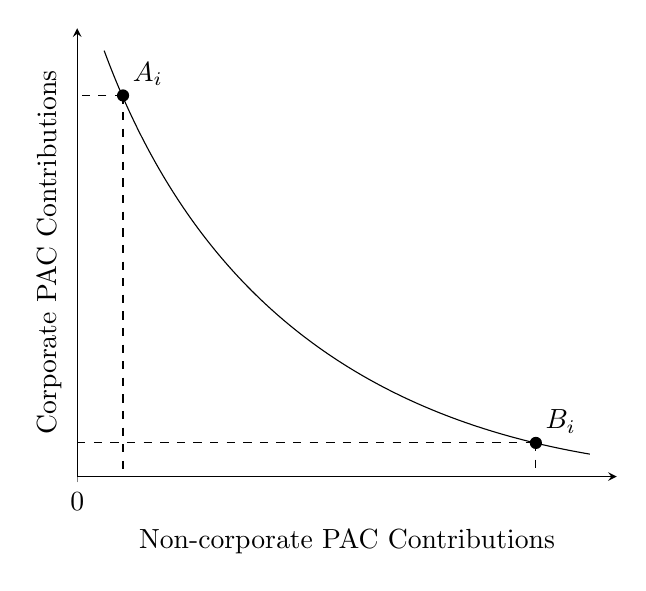
\begin{tikzpicture}
\begin{axis}[
    axis x line=bottom,
    axis y line=left,
    xmin=0, xmax=10, 
    ymin=0, ymax=10,
    xlabel={Non-corporate PAC Contributions},
    ylabel={Corporate PAC Contributions},
    ytick=\empty,
    xtick={0},
    extra y tick style={align=center, font=\scriptsize},
    ]
    \draw (axis cs:0.5,9.5) to [bend right=30] coordinate[pos=0.2] (l_i) (axis cs:9.5,0.5);
    \fill (axis cs:0.85,8.5) circle (2.2pt) node[above right] {$A_i$};

    \fill (axis cs:8.5,0.75) circle (2.2pt) node[above right] {$B_i$};
    
    \draw[dashed, thin] (axis cs:0.85,8.5) -- (axis cs:0.85,0);
    \draw[dashed, thin] (axis cs:0.85,8.5) -- (axis cs:0,8.5);
    \draw[dashed, thin] (axis cs:8.5,0.75) -- (axis cs:8.5,0);
    \draw[dashed, thin] (axis cs:0,0.75) -- (axis cs:8.5,0.75); 
\end{axis}
\end{tikzpicture}
\caption{\textbf{Campaign Contribution Decision Trade-off.} This figure presents an isoquant map of the combination of campaign contributions needed to reach a winning vote threshold of 51 percent. Candidates at $A_i$ use more corporate PAC contributions while candidates at $B_i$ use more non-corporate PAC contributions to accomplish the same 51 percent threshold.}
\label{fig: iso map}
\end{figure}
 
 In summary, pledging to reject corporate PAC contributions likely signals to voters that a candidate is not ``bought-out" by special interests and is thus more trustworthy. As a result of this signaling, the candidate should receive an increase in individual small-dollar donations. Rejecting such a significant source of funding also introduces an electoral risk, one that political parties, who are primarily interested in the success of their candidates, may be unwilling to accept. Thus, candidates who reject PAC money will receive an increase in contributions from partisan organizations like political parties themselves or other elected officials. Finally, since the opportunity cost of not making political contributions is so high \citep{grier1991}, corporations are unlikely to cease their involvement in campaign funding because a member will not accept money from their associated PAC. Instead, they could still exert their influence, albeit more discreetly, through individual donations. Thus, candidates that pledge to reject corporate PAC contributions will receive an increase in contributions from individuals associated with corporations.


\section{Data}

To test these hypotheses, I use campaign finance data on Congressional candidates in the 2018 midterm election provided by The Center for Responsive Politics at \href{https://www.opensecrets.org}{Opensecrets.org.} Because data on which candidates did and did not pledge to reject corporate PAC donations is incomplete, I am only using a sample of 2018 candidates. Next, to facilitate better comparison groups, I restrict the sample to only Democrats who won their election. Since the composition of campaign contributors differs between parties, only including Democrats helps to remove some of this heterogeneity. Second, it is necessarily the case that candidates that did not win their elections differ, likely systematically, from those that did win, and these differences could be on factors that also determine campaign contributions. By excluding losers from the sample, these differences are effectively controlled for. Not do these restrictions help with comparisons, but of the 539 candidates with data on pledges, there are only 2 Republicans that took the pledge to reject corporate PAC contributions. Thus, the final sample contains 167 Democratic candidates that won election in their district. Although this produces helpful comparison groups, my ability to make causal inferences is still limited. I do not claim to have identified causal effects. Instead, this study is an effort to understand the associational patterns of campaign contribution activity for candidates that do and do not accept corporate PAC contributions. 

In addition to campaign finance data, I also use vote share data for each candidate from the \href{https://electionlab.mit.edu/data}{MIT Election Data + Science Lab}. Finally, I get Congressional district demographic data from the U.S. Census Bureau.  

\begin{figure}[!htb]
    \centering
    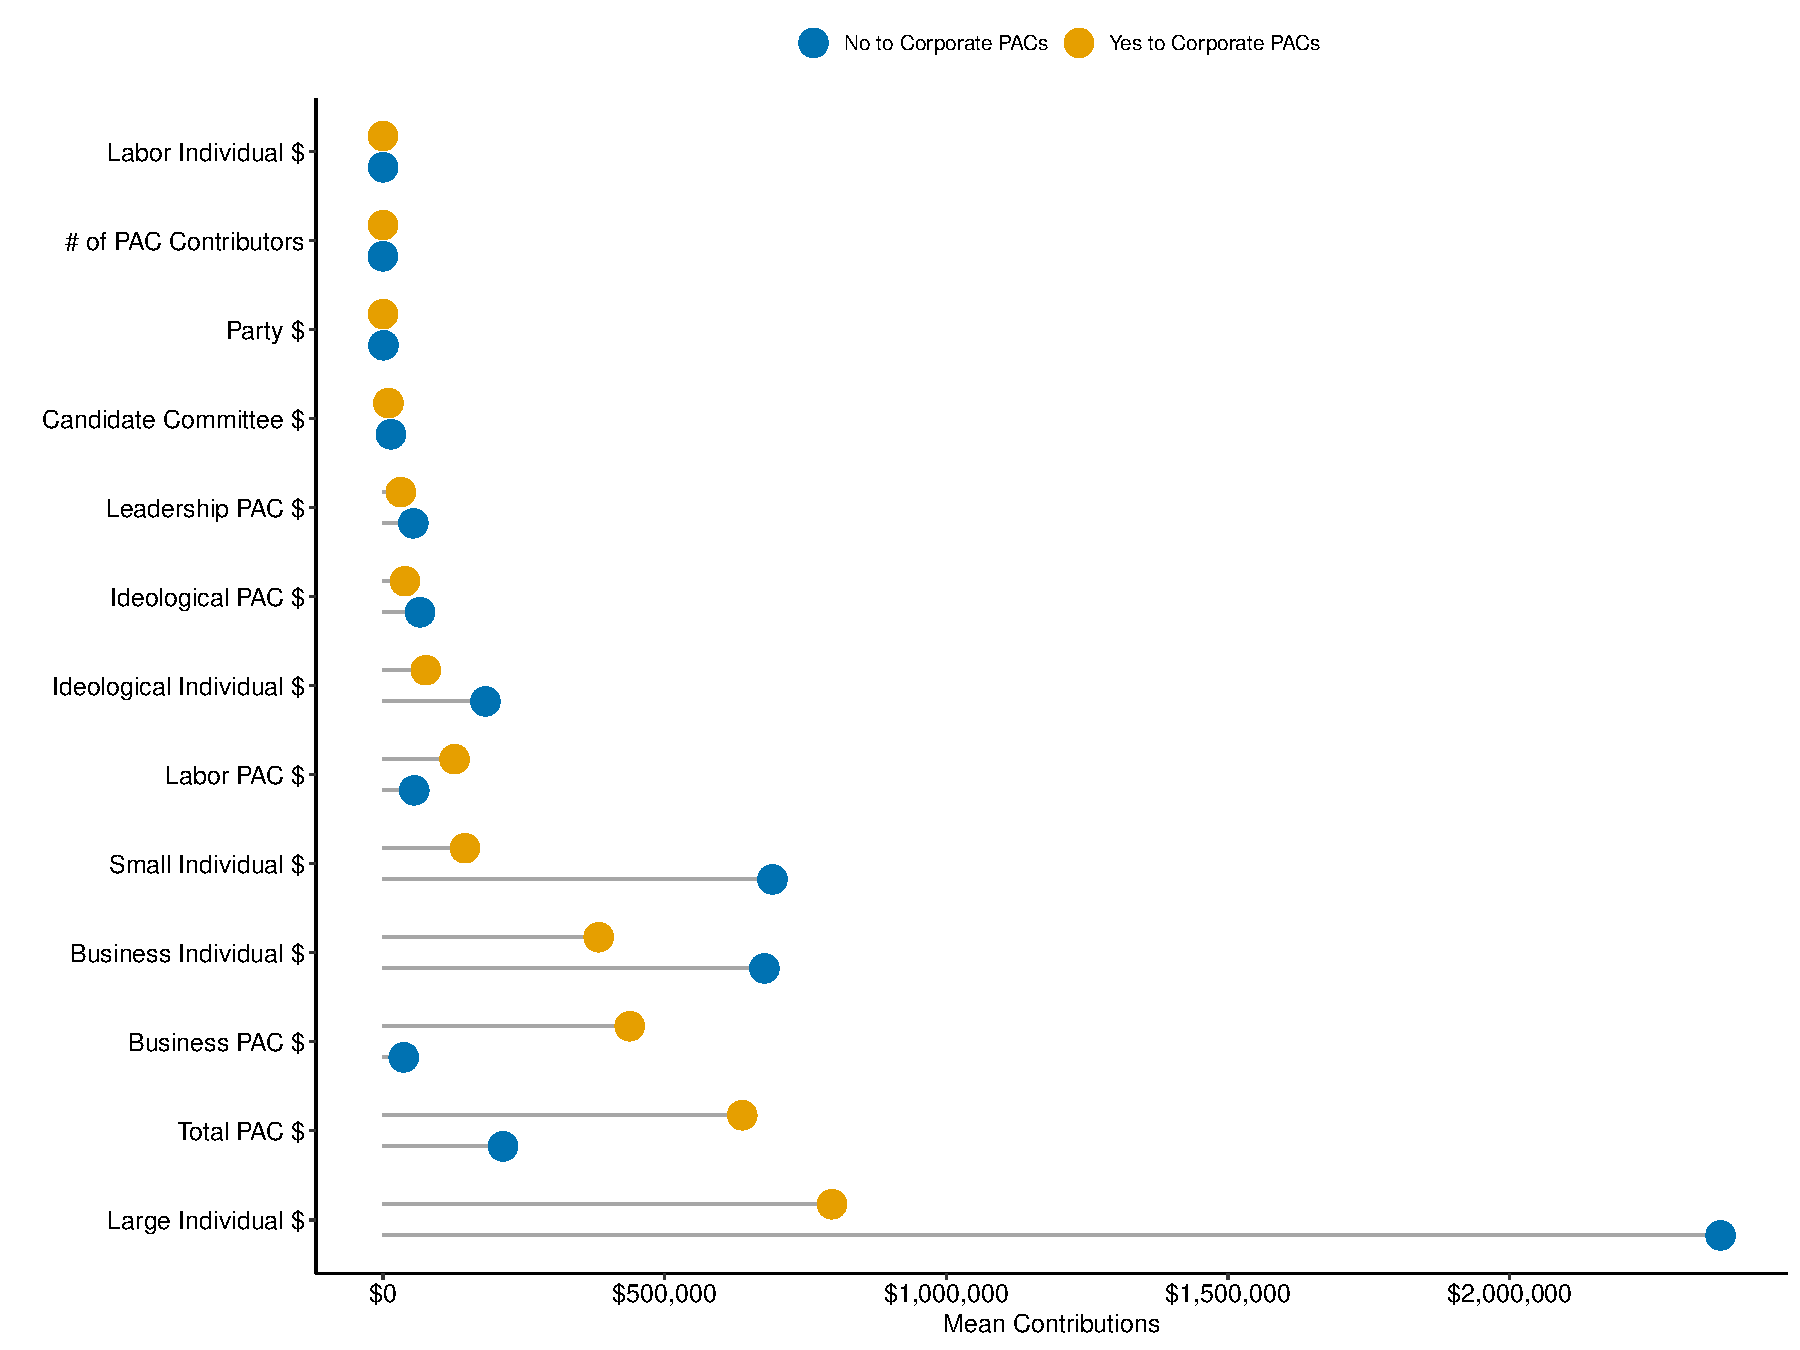
\includegraphics[width=0.90\linewidth]{../../Figures/all_candy.pdf}
    \caption{\textbf{Contributions to Candidates by Source and Whether or not they Reject PAC Contributions.} This figures shows that while candidates who pledge to reject corporate PAC contributions receive fewer contributions from business PACs, they receive more contributions from leadership PACs, ideological PACs, individuals affiliated with ideological interest groups, small-dollar donations, individuals affiliated with business interest groups, and large-dollar donations.}
    \label{fig: all contribs}
\end{figure}

Figure \ref{fig: all contribs} displays the mean contributions across candidates by whether or not they pledge to reject corporate PAC contributions. We see that candidates who pledge to reject corporate PAC contributions receive almost zero contributions from business PACs, and they also receive much fewer contributions from PACs in total. However, these candidates also receive more contributions from leadership PACs, ideological PACs, individuals affiliated with ideological interest groups, small-dollar donations, individuals affiliated with business interest groups, and large-dollar donations.

\begin{figure}[ht]
    \centering
    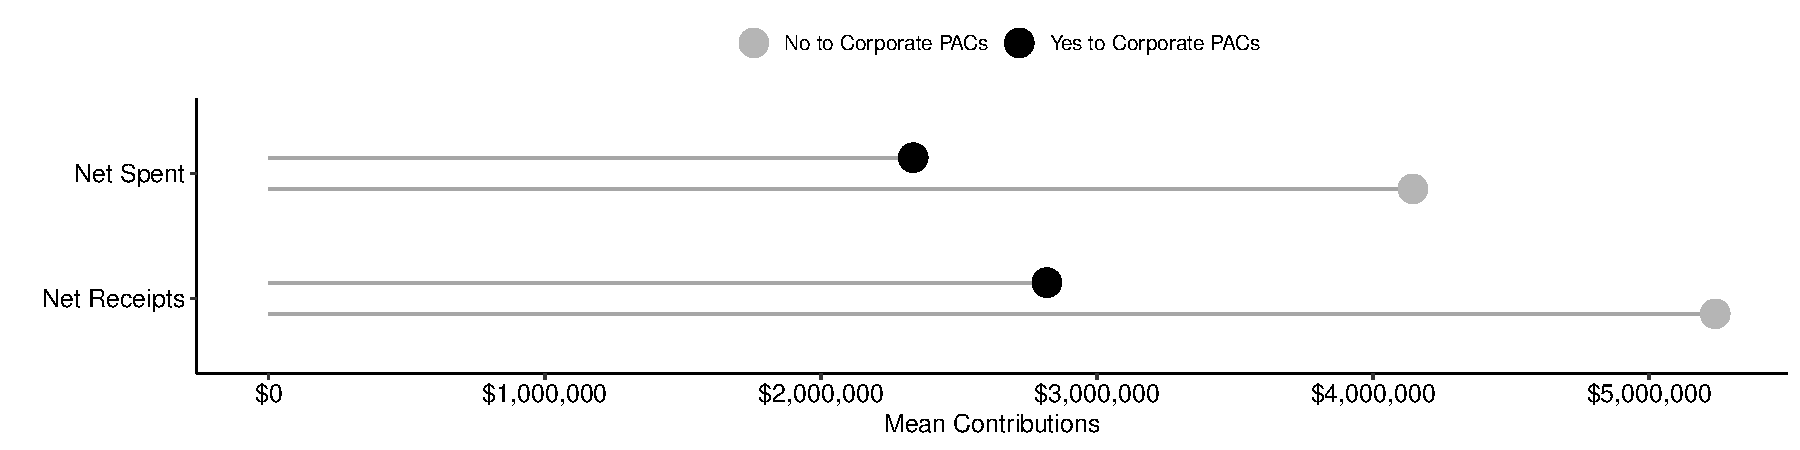
\includegraphics[width=0.90\linewidth]{../../Figures/spending_candy.pdf}
    \caption{\textbf{Mean Candidate Spending and Receipts by Whether or not they Reject PAC Contributions.} This figure shows that candidates who pledge to reject corporate PAC contributions spend about 2.5 times more than their PAC accepting counterparts and receive about 2.25 times more total contributions.}
    \label{fig: spending}
\end{figure}

Figure \ref{fig: spending} displays the mean level of campaign spending and receipts by whether or not the candidate pledges to reject corporate PAC contributions. Here we see that candidates who reject corporate PAC contributions outspend and out-raise their PAC-accepting counterparts by a significant margin.


\section{Model Definition}

The goal of any statistical model is to describe the data generating process of the outcome under consideration. In this study, the primary interest is in modeling the generative process of campaign contributions from PACs, political party organizations, and individuals. Campaign contributions are composed of positive real values. Thus, campaign contributions likely arise from a gamma process since the gamma distribution describes a data generating process for a random variable with only positive real number outcomes $y \in  \mathbb{R}^+$. 

However, because some candidates pledge to reject contributions from PACs, contribution values of zero are also possible. A zero could result because they accept zero contributions from a group, but a group could also decide not to contribute to a candidate because they pledged to reject PAC contributions. For example, suppose a new candidate takes to pledge to reject PAC contributions because they feel that doing so is morally right. Further suppose, however, that their political party's leadership wanted the candidate to announce their opposition to PACs after they had some time to evaluate this candidate's probability of winning the election and estimate their fundraising needs. Because the candidate did not wait for the party's approval, the party decides that this candidate has little chance of success given the timing of their announcement and therefore chooses not to give this candidate funds from the party committee. In this situation, the candidate would receive zero contributions from their party because they pledge to reject PAC contributions. This dual process is summarized in Figure \ref{fig: zeros}. Candidates decided either to reject PACs with probability of $\pi$ or accept PACs with probability $(1 - \pi$). If they reject PACs, we will observe a zero. If they do not reject PACs, we may still observe a zero if the candidate fails to attract donations from the group in question. 

\begin{figure}[!htb]
    \centering
    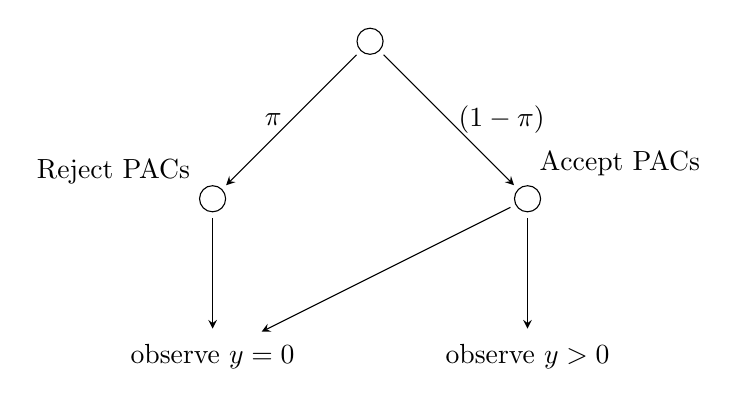
\begin{tikzpicture}[
        node distance=2.0cm,
      scale=0.5,
      level/.style={thick},
      virtual/.style={thick,densely dashed},
      trans/.style={->,shorten >=2pt,shorten <=2pt,>=stealth},
      classical/.style={thin,double,<->,shorten >=4pt,shorten <=4pt,>=stealth}
    ]
    \node(a)[circle, draw=black, label={160:Reject PACs}] {};
    \node(z)[right of=a] {};
    \node(b)[circle, draw=black, right of=z, label={80:Accept PACs}] {};
    \node(c)[circle, draw=black, above of=z] {};
    \node(d)[below of=a] {observe $y = 0$};
    \node(e)[below of=b] {observe $y > 0$};
    
    \draw [trans] (c) -- (a) node[midway, left] {$\pi$};
    \draw [trans] (c) -- (b) node[midway, right] {$(1 - \pi)$};
    \draw [trans] (a) -- (d);
    \draw [trans] (b) -- (e);
    \draw [trans] (b) -- (d);
    \end{tikzpicture}
    \caption{\textbf{Zero Generation Process.} Candidates can receive zero contributions through two different process. First, they may receive zero contributions because they pledge to reject PAC contributions. Second, they may receive zero contributions because they simply do not receive contributions from a particular group.}
    \label{fig: zeros}
\end{figure}

Figure \ref{fig: zeros} shows the percentage of zeros in the data. Of the 167 candidates in the data, 84 percent did not receive contributions from party committees, 68 percent did not receive contributions from individuals affiliated with labor organizations, 12 percent did not receive contributions from candidate committees, 10 percent did not receive contributions from leadership PACs, 5 percent did not receive contributions from business PACs,  4 percent did not receive contributions from individuals affiliated with ideological organizations, 2 percent did not receive contributions from labor PACs, and 1 percent did not receive contributions from ideological PACs and PACs in general.  

\begin{figure}[!htb]
    \centering
    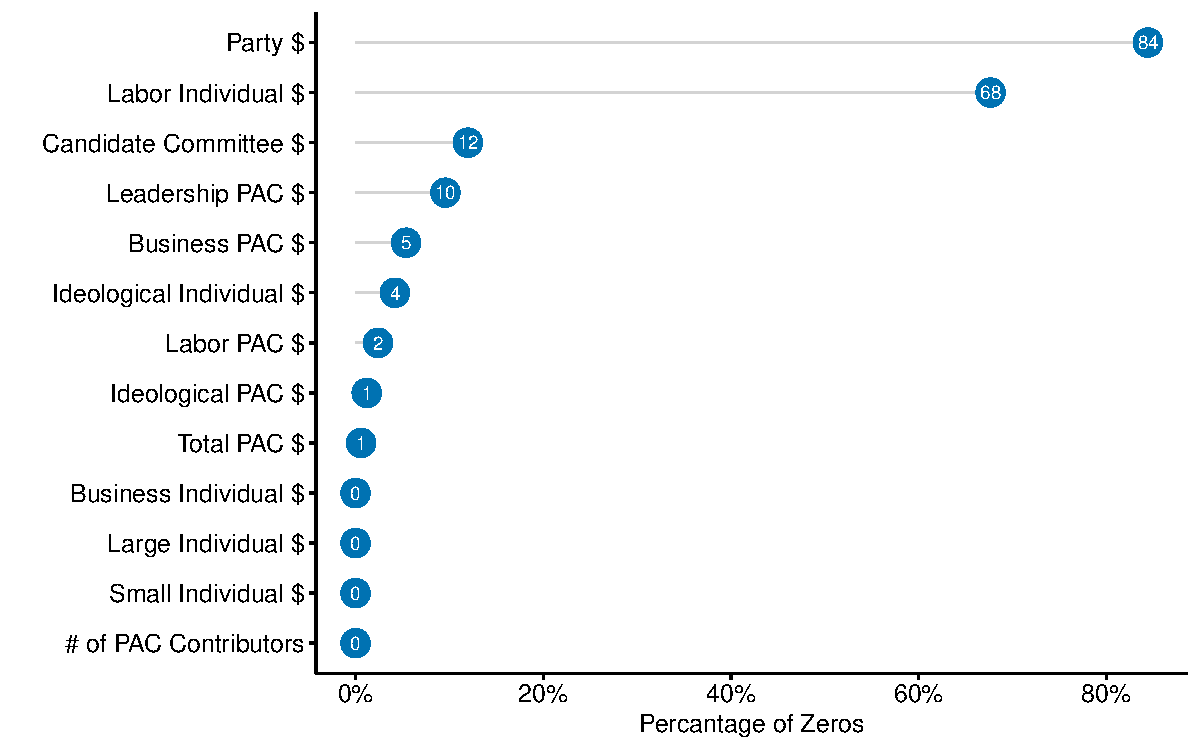
\includegraphics[width=0.85\linewidth]{../../Figures/zero_candy.pdf}
    \caption{\textbf{Percentage of Zero Contributions in the Data by Source of Contribution.}}
    \label{fig: zeros}
\end{figure}

Because the gamma distribution is not defined for zero values, I use a zero-augmented gamma likelihood function for models of contributions that contain zero values as mentioned above. The zero-augmented gamma likelihood is a mixture of a bernoulli and gamma process. Thus, the probability density $f(y)$ for contributions can be defined as:    

\begin{align}
f(y) = \left\{ \begin{array}{cc} 
                \pi & \hspace{5mm} \text{if $y = 0$} \\
                (1 - \pi) \text{Gamma}(k, \theta) & \hspace{5mm}  \text{if $y > 0$} \\
                \end{array} \right.
\end{align}

\noindent where $\pi$ is the probability of receiving zero contributions from a given group ($y = 0$), and $k$ and $\theta$ define a gamma distribution with mean $k\theta^{-1}$ and rate $\theta$. This likelihood can be easily summarized as $\text{ZGamma}(\pi, \mu, \theta)$ where $\pi$ indicates the probability of a zero, and non-zero outcomes are described by a mean $\mu$ and rate $\theta$. For more information on the mathematical details, see \citet{mccullagn1989}. An alternative solution to model this data would be to model cases of zero contributions separately from non-zero cases, but this approach would sacrifice information about the relationship between these cases. By leaving zero cases in the dataset, the model can allow the probability of observing a zero inform the coefficient estimates in the gamma likelihood and vice versa. This way, the model can develop a more accurate picture of the data generating process.

Although this pooling of information leads to more informative estimates, this can only be the case if there are enough zero cases to provide useful information. As a result, it is unlikely that the model will learn anything meaningful for the cases where the occurrence of zeros is between 1 and 5 percent, even 12 percent is doubtful. For these models, the estimated probability of observing a zero will almost certainly be determined by the priors simply because there is not enough data. By using weakly-informative priors, we can extract some useful information, but ultimately the model will benefit very little from retaining the zeros in the data. In these cases, the estimated effect of rejecting PACs on contributions will converge to the gamma likelihood estimates. 

\subsection{Modeling Campaign Contributions}

Campaign contributions are divided into three groups—contributions from PACs, contributions from political party organizations, and contributions from individuals. In the PAC group, I examine the pattern of contributions made to candidates from PACs that primarily represent business, labor, and ideological interests. In the political party group, I examine contributions to candidates from leadership PACs, political party committees, and candidate committees. Leadership PACs are PACs created by incumbents to raise money to cover expenditures that cannot be paid by campaign committees or congressional offices. Additionally, leadership PAC funds can be used to fund other candidates' campaigns, as is often the case \citep{herrnson2009, lazer2015}.

Along with leadership PACs, political parties can also contribute to a candidate's campaign. Finally, a member can use their candidate committee to contribute to another member's campaign. This is often done to support candidates of one's party who are challenging incumbents or are at risk of being defeated \citep{wilcox1989, lazer2015a}. 

For the final group, individual contributions, I examine small-dollar contributions ($< \$200$), large-dollar contributions ($> \$200$), and individual contributions associated with ideological, labor, and business organizations. Since the Federal Election Commission requires that all contributions above \$200 must be itemized and list the donor's employer and occupation information, this information can be used to approximate a donor's economic interest. This is, of course, not a perfect measurement, but it will provide insight into the types of individual donations that a candidate receives. 

The model structure used to estimate campaign contributions for outcomes that contain zeros is given by: 

$$
\begin{aligned}
    y_i &\sim \text{ZGamma}(\pi_i, \mu_i, \theta_i) \\
    \log \frac{\pi_i}{1 - \pi_i} &= \alpha_{\pi} + \beta_{1\pi} (\text{No PACs})_i + \beta_{2\pi} (\text{New Member})_i \\
    \log(\mu_i) &= \alpha_{\mu} + \beta_{1\mu} (\text{No PACs})_i + \bm{X} \bm{\beta_{\mu}} \\
\end{aligned}
$$

\noindent where $i$ indexes individuals, $\bm{X}$ is a matrix of control variables, and $\bm{\beta_{\mu}}$ is the corresponding coefficient vector. In these models, the probability of receiving contributions is modeled as a function of both rejecting PACs (0 - 1 indicator) and being a new member (0 - 1 indicator). Previous research indicates that PACs almost exclusively contribute to incumbents \citep{brunell2005} and that they often wait to support challengers until they show success in raising funds from other sources \citep{biersack1993}. 

To model campaign contributions for outcomes without zeros (small-dollar individual, large-dollar individual, business individual, total individual, vote share, voting-age population turnout), I use a standard gamma likelihood.

\subsection{Priors}

Just as the choice of likelihood and link functions can lead to different results, the choice of priors also affects model results. Priors, even when somewhat strong, are typically overridden by the data when working with large-n dataset, but when working with small-n data, priors can have large influences if one is not careful \citep{mcneish2016}. Although this risk is present, Bayesian methods can also outperform Frequentist methods when working with small-n data since Bayesian analysis does not rely on asymptotic properties and because priors can be used to help narrow the range of plausible values that the model can produce. 

I use weakly-informative priors for two reasons. First, because the sample size is 167 individuals, I use priors to inform the model of what values the parameters can reasonably take on. This practice leads to estimates that better approximate large-n estimates because of irregular variance due to the small-n nature of the data can be discounted \citep{mcneish2016}. Second, using ``uninformative" priors is seldom justified since one always knows something \textit{a priori} about the range of plausible values \citep{gelman2008a}. For example, whether one studies politics or not, it is known that a candidate's vote share cannot exceed 100 percent and cannot fall below 0 percent. For simulations of the priors used in each specification, see Appendix \ref{sec: prior sims}.


\section{Results}

\subsection{Contributions from PACs}

In examining the effects of rejecting corporate PAC contributions, I start by investigating how the pledge affects contribution patterns from business, labor, and ideological PACs. The results from these estimations are summarized in Figure \ref{fig: pac results}. Figure \ref{fig: pac coefs} presents the estimates for non-zero contributions and shows that pledging to reject corporate PAC contributions is associated with a decrease in PAC contributions from businesses, labor interest groups, and ideological interest groups. Interestingly, however, for zero contributions, Figure \ref{fig: pac probs} shows that pledging to reject corporate PAC contributions increases the probability of not receiving contributions from business PACs only. This suggests that while \emph{how much} ideological and labor PACs contribute depends on whether or not they reject corporate PAC contributions, \emph{whether or not} they give does not. 

\begin{figure*}[!htb]
    \centering
    \begin{subfigure}[b]{0.65\textwidth}
        \centering
        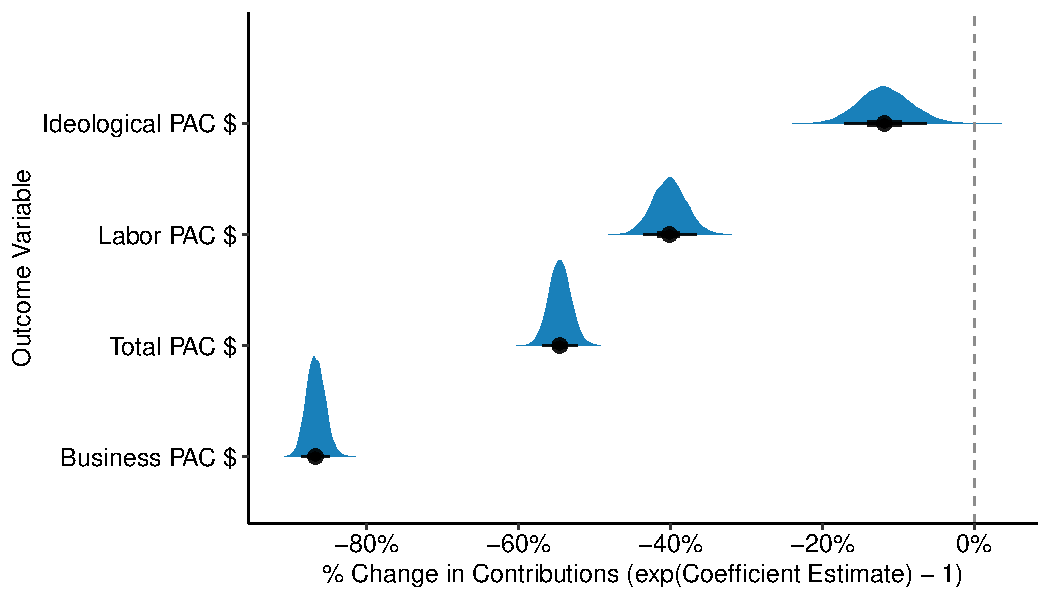
\includegraphics[width=1\linewidth]{../../Figures/Results/pac_coef.pdf}
        \caption{The Effect of Rejecting Corporate PAC Contributions on PAC Contributions.}
        \label{fig: pac coefs}
    \end{subfigure}
    
    \begin{subfigure}[b]{0.65\textwidth}
        \centering
        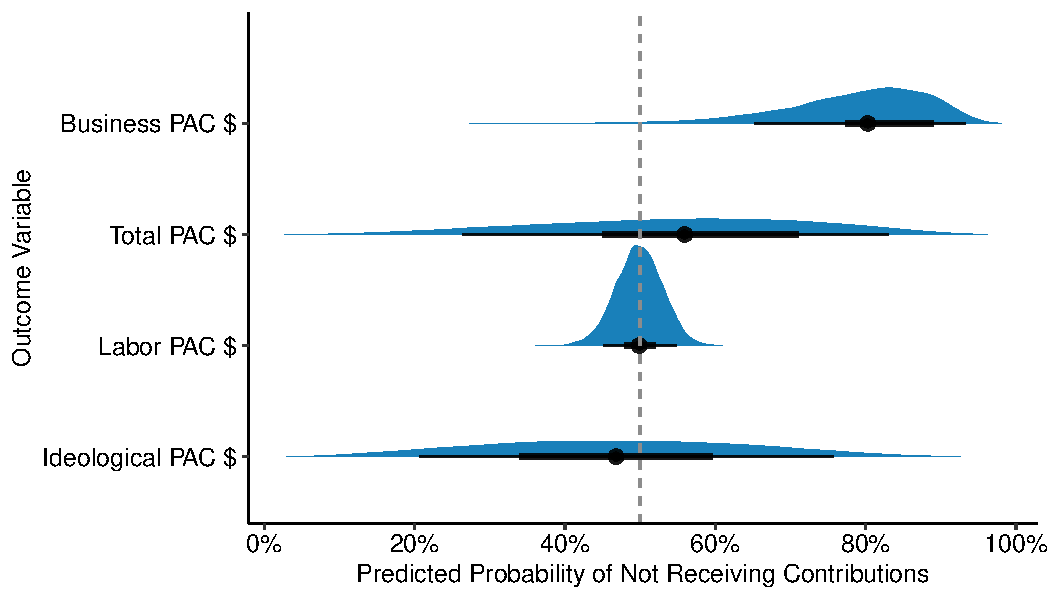
\includegraphics[width=1\linewidth]{../../Figures/Results/pac_probs.pdf}
        \caption{The Effect of Rejecting Corporate PAC Contributions on the Probability of Receiving PAC Contributions}
        \label{fig: pac probs}
    \end{subfigure}
    \caption{\textbf{The Effect of Rejecting Corporate PAC Contributions on PAC Contributions and the Probability of Receiving Money from PACs.} These figures present the posterior distributions estimated for a candidate that pledges to reject corporate PAC contributions. The dot shows the median coefficient estimate and the intervals show the 50\% and 89\% highest density intervals. Figure \ref{fig: pac coefs} shows that candidates that pledge to reject corporate PAC contributions experience a reduction in contributions from all types of PACs. Figure \ref{fig: pac probs} shows that rejecting corporate PAC contributions increases the probability of not receiving contributions from business PACs. See Table \ref{tbl: pac results} for the formal estimates.}
    \label{fig: pac results}
\end{figure*}

Candidates who pledge to reject corporate PAC contributions receive fewer contributions from ideological, labor, and business PACs, but is it enough to matter? Figure \ref{fig: pac preds} shows the total amount of contributions each candidate type is predicted to receive by PAC category. For ideological PACs, the predicted difference of roughly \$3,000 is negligible, but the differences for labor and business PAC contributions are more substantial. Candidates that pledge to reject corporate PAC contributions are predicted to receive about \$47,000 less than candidates who do not take the pledge. For business PACs, the difference is about \$358,000 - a substantively meaningful difference.  

\begin{figure*}[!htb]
    \centering
    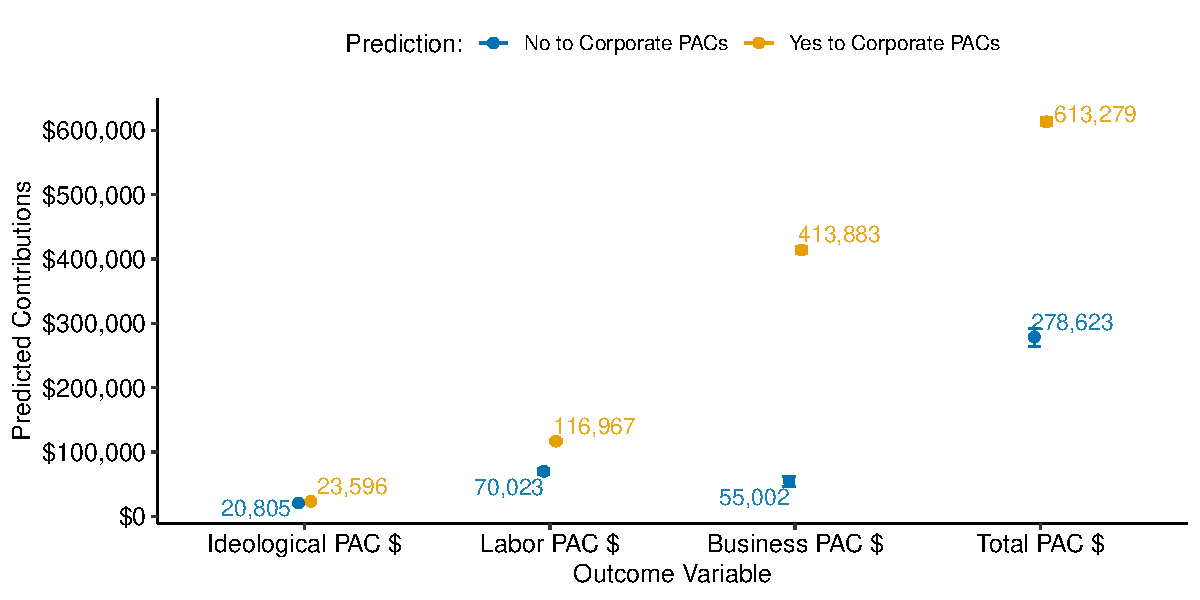
\includegraphics[width=1\linewidth]{../../Figures/Results/pac_preds.pdf}
    \caption{\textbf{Total Predicted Contributions from Each PAC by Candidate Type.} This figure shows that candidates who pledge to reject PAC contributions are predicted to received fewer contributions from PACs, but the difference is largest for contributions from business PACs.}
    \label{fig: pac preds}
\end{figure*}


\subsection{Contributions from Party Organizations}

The second category of contributions I examine are those from political party organizations. Specifically, I examine contributions from candidate committees, political party committees, and leadership PACs. Once a candidate for office spends or receives more than \$5,000, they become an official candidate and must establish a campaign committee, called a ``candidate committee," to receive contributions and make campaign expenditures. Once in office, members retain their candidate committees for reelection purposes, but they also use them to support other candidate's electoral efforts. Typically, members transfer funds between candidate committees to help incumbents retain their seats or challengers unseat members from the opposing party. 

Leadership PACs are established by members after elections to raise money for their future political career prospects. They are typically used to pay for expenses that campaign committee funds cannot be used for, but, much like candidate committees, they are also used to support fellow candidates. 

\begin{figure*}[!htb]
    \centering
    \begin{subfigure}[b]{0.65\textwidth}
        \centering
        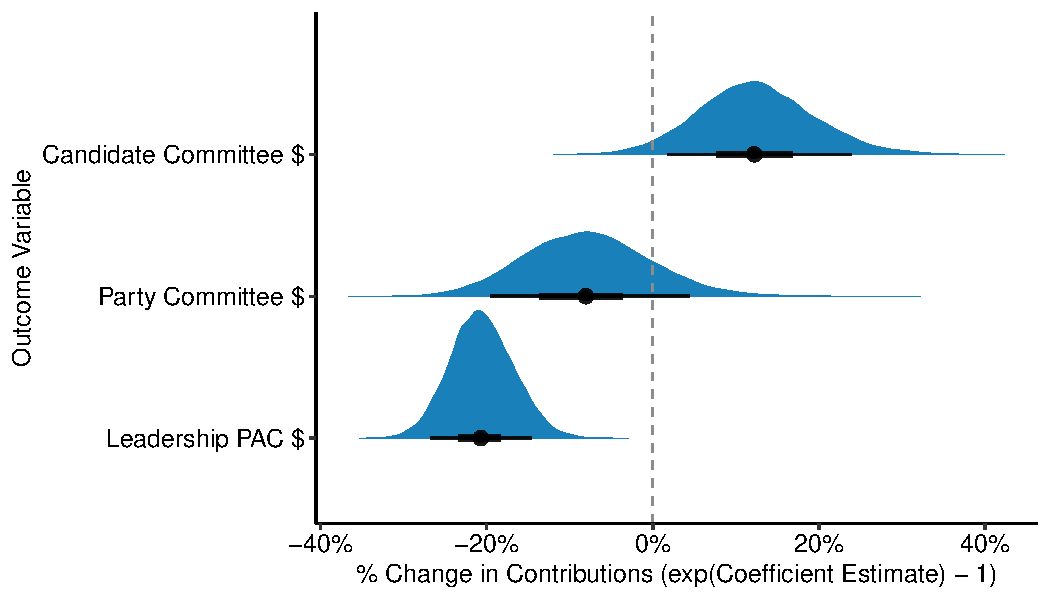
\includegraphics[width=1\linewidth]{../../Figures/Results/party_coef.pdf}
        \caption{The Effect of Rejecting Corporate PAC Contributions on Contributions from Party Organizations.}
        \label{fig: party coefs}
    \end{subfigure}
    
    \begin{subfigure}[b]{0.65\textwidth}
        \centering
        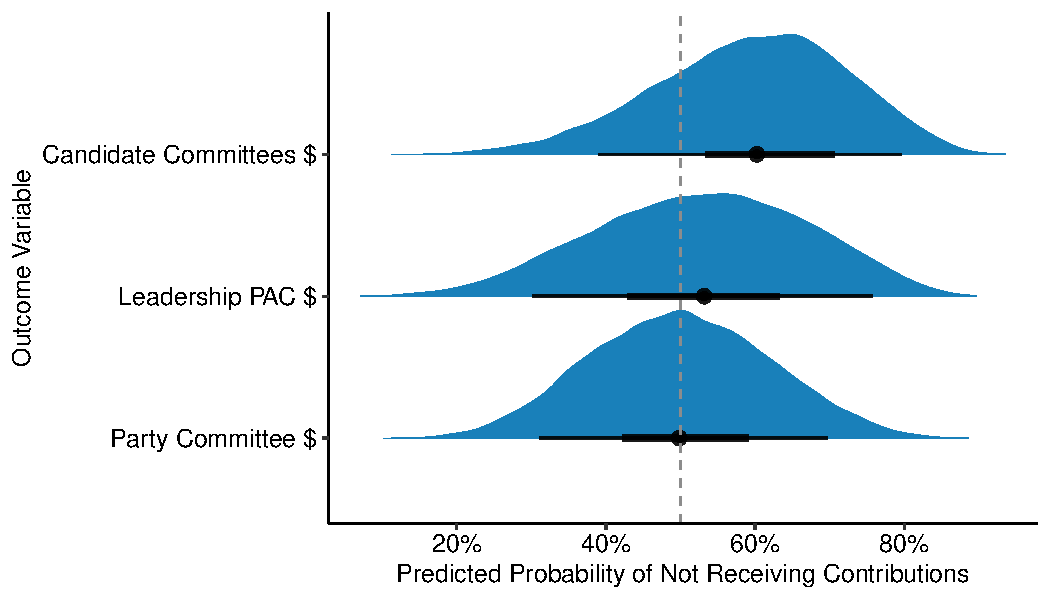
\includegraphics[width=1\linewidth]{../../Figures/Results/prty_probs.pdf}
        \caption{The Effect of Rejecting Corporate PAC Contributions on the Probability of Receiving Party Contributions.}
        \label{fig: party probs}
    \end{subfigure}
    \caption{\textbf{The Effect of Rejecting Corporate PAC Contributions on Contributions and the Probability of Receiving Money from Political Parties.} These figures present the posterior distributions estimated for a candidate that pledges to reject corporate PAC contributions. The dot shows the median coefficient estimate and the intervals show the 50\% and 89\% highest density intervals. Figure \ref{fig: party coefs} shows that candidates that pledge to reject corporate PAC contributions experience a reduction in contributions from leadership PACs but also experience an increase in contributions from candidate committees. Figure \ref{fig: party probs} shows that rejecting corporate PAC contributions has no effect on the probability of receiving contributions from candidate committees, leadership PACs, or political parties. See Table \ref{tbl: party results} for the formal estimates.}
    \label{fig: party results}
\end{figure*}

Finally, political parties also have their own PACs that are used to support their party's candidates either directly or indirectly. Because rejecting corporate PAC money may be done strategically because a candidate knows that they will have support from party organizations, I examine each of these sources individually.  

The results from these models are presented in Figure \ref{fig: party results}. Figure \ref{fig: party coefs} displays the estimates for non-zero contributions and shows that candidates who reject corporate PAC contributions receive more contributions from candidate committees and fewer contributions from leadership PACs. Although I am unable to test for causal effects, this could be indicative of a strategic motivation for taking the pledge. Candidates who pledge to reject corporate PAC contributions could do so because they know they will receive financial support from other candidates. With respect to whether or not taking the pledge affects the probability of receiving contributions from these categories, Figure \ref{fig: party probs} indicates that it has no effect. Much like the previous findings, this means that pledging to reject corporate PAC donations is associated with changes in \emph{how much} a candidate receives from these groups, but it is not associated with \emph{whether or not} these groups contribute to an individual's campaign. 

Again, however, it is important to assess the substantive importance of the contribution changes. The total predicted contributions from candidate committees, leadership PACs, and party committees are presented in Figure \ref{fig: party preds}. Although the model for candidate committee contributions estimates that rejecting corporate PACs likely has a non-zero relationship with contributions, it predicts that these candidates will receive about \$400 more than candidates who do not take the pledge. Such an amount is likely inconsequential, but it is still consistent with the possibility that the pledge is taken for strategic reasons. Perhaps none of the candidates needed to accept the agreed-upon money from other candidates because funds from other sources exceeded expectations. 

The story is a bit different with leadership PACs. Here, the model predicts that candidates who take the pledge will receive about \$2,500 less than candidates who do not take the pledge. Such a difference could make a difference in a marginal race, perhaps, but it is nonetheless a rather small amount.    

\begin{figure*}[!htb]
    \centering
    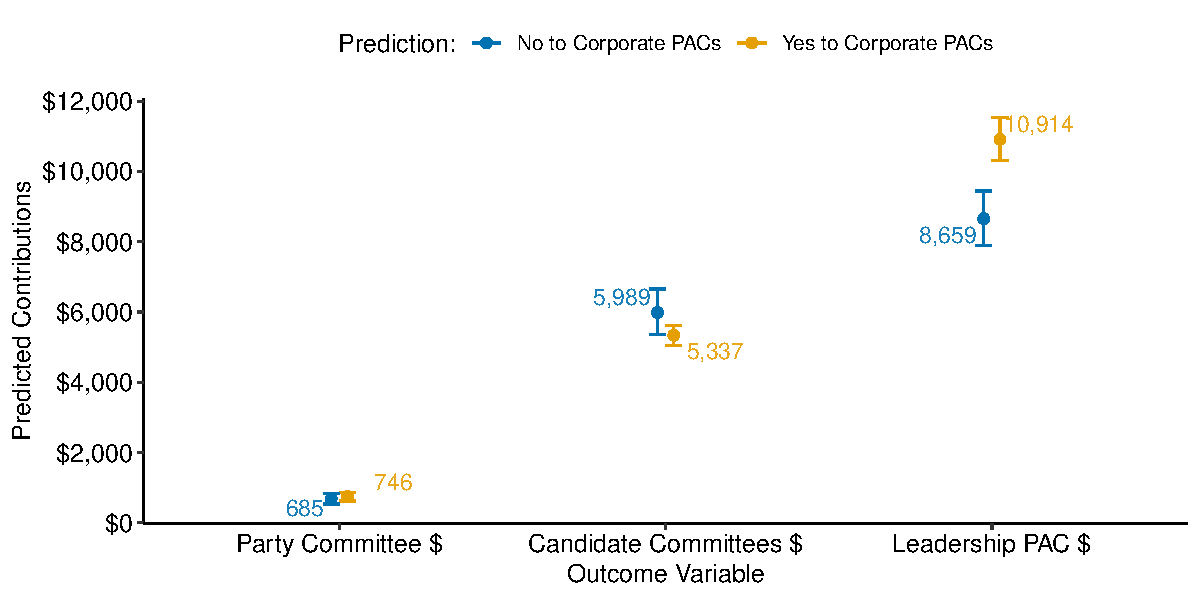
\includegraphics[width=1\linewidth]{../../Figures/Results/party_preds.pdf}
    \caption{\textbf{Total Predicted Contributions from Each Party Organization by Candidate Type.} This figure shows that candidates who pledge to reject PAC contributions are predicted to received fewer contributions from leadership PACs but more contributions from candidate and party committees.}
    \label{fig: party preds}
\end{figure*}

\subsection{Contributions from Individuals}

The final category of contributions that I examine are those from individual donors. Candidates who reject corporate PAC contributions frequently advertise this fact in an apparent attempt to increase the number of small-dollar contributions they receive from individuals. Consistent with their expectations, Figure \ref{fig: indiv coefs} offers supporting evidence. Remarkably, candidates who pledge to reject corporate PAC contributions receive over a 90 percent increase in contributions from donations less than \$200. It appears that this is an effective strategy to increase small-dollar donations from individuals. 

Interestingly, campaign contributions from individuals affiliated with businesses, ideological organizations, and large-dollar contributions increase as well. This suggests that when candidates pledge to reject corporate PAC contributions, interest groups might channel their contributions through individual donors. This finding is shown more clearly in Figure \ref{fig: indiv preds}. 

\begin{figure*}[!htb]
    \centering
    \begin{subfigure}[b]{0.65\textwidth}
        \centering
        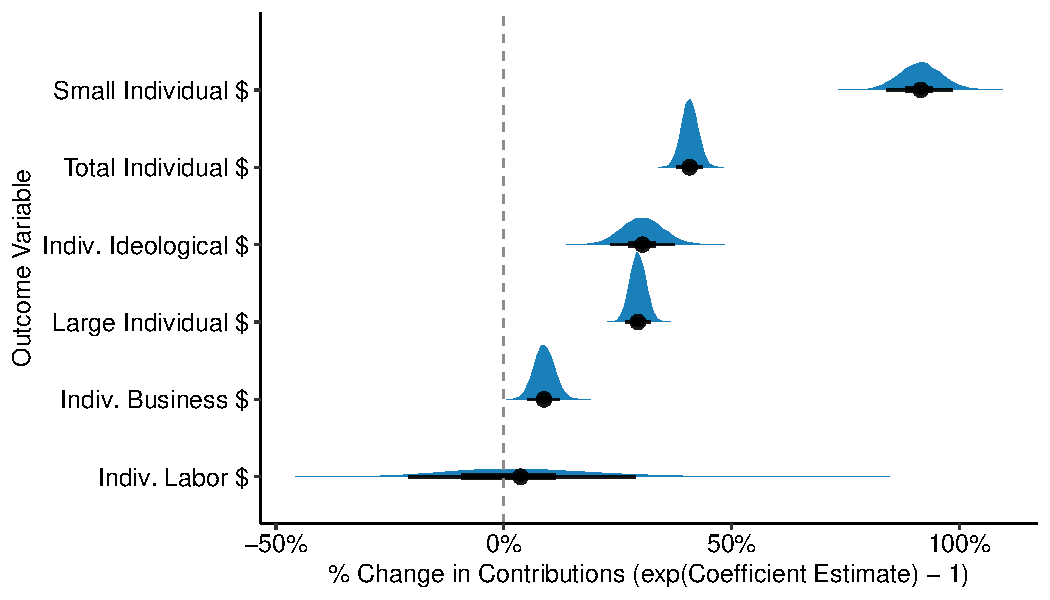
\includegraphics[width=1\linewidth]{../../Figures/Results/indv_coef.pdf}
        \caption{The Effect of Rejecting Corporate PAC Contributions on Contributions from Individuals.}
        \label{fig: indiv coefs}
    \end{subfigure}
    
    \begin{subfigure}[b]{0.65\textwidth}
        \centering
        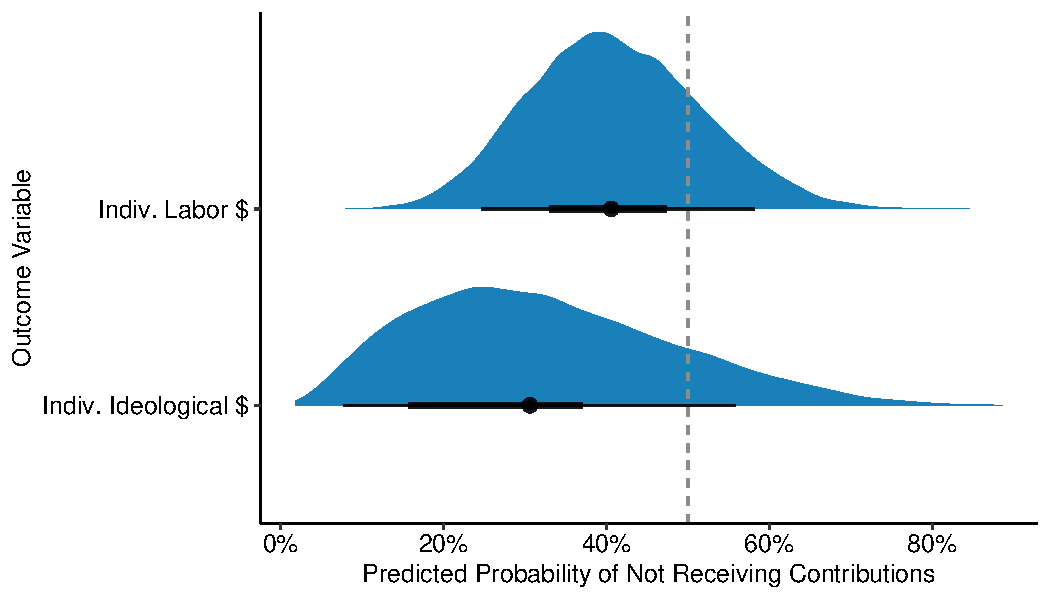
\includegraphics[width=1\linewidth]{../../Figures/Results/indiv_probs.pdf}
        \caption{The Effect of Rejecting Corporate PAC Contributions on the Probability of Receiving Individual Contributions.}
        \label{fig: indiv probs}
    \end{subfigure}
    \caption{\textbf{The Effect of Rejecting Corporate PAC Contributions on Contributions and the Probability of Receiving Money from Individuals.} These figures present the posterior distributions estimated for a candidate that pledges to reject corporate PAC contributions. The dot shows the median coefficient estimate and the intervals show the 50\% and 89\% highest density intervals. Figure \ref{fig: indiv coefs} shows that candidates that pledge to reject corporate PAC contributions experience an increase in contributions from small-dollar, total, ideological, large-dollar, and business individual contributions. Figure \ref{fig: indiv probs} shows that rejecting corporate PAC contributions has no effect on the probability of receiving contributions from individuals affiliated with labor or ideological interest groups. See Table \ref{tbl: indiv results} for the formal estimates.}
    \label{fig: indiv results}
\end{figure*}

Figure \ref{fig: indiv preds} shows that candidates who take the pledge to reject corporate PAC contributions receive an increase in contributions of roughly \$10,000, \$50,000, \$24,000, and \$145,000 from individuals affiliated with ideological interest groups, donations less than \$200, individuals affiliated with businesses, and donations larger than \$200, respectively. 

Figures \ref{fig: indiv coefs} and \ref{fig: indiv preds} indicate that voters hoping that candidates who do not accept corporate PAC contributions are more ``trustworthy" concerning their campaign funding should not hold their hopes firmly. These results are consistent with what one would expect if pledges to reject corporate PAC contributions are strategies to get voters to think that they are more honest candidates while continuing to accept donations from corporate interests through alternative sources. 
 
\begin{figure*}[!htb]
    \centering
    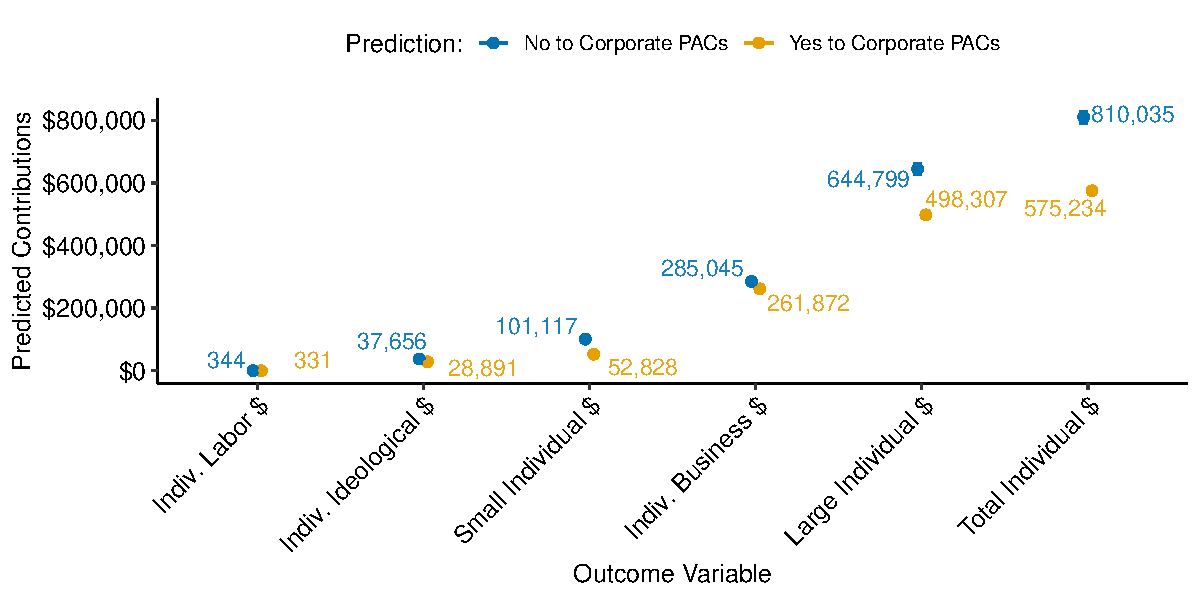
\includegraphics[width=1\linewidth]{../../Figures/Results/indv_preds.pdf}
    \caption{\textbf{Total Predicted Contributions from Individuals by Candidate Type.} This figure shows that candidates who pledge to reject PAC contributions are predicted to received more contributions from individuals affiliated with ideological and business interests, as well as contributions less than and greater than \$200.}
    \label{fig: indiv preds}
\end{figure*}


\subsection{Voting Effects}

Finally, if rejecting corporate PAC contributions increases, small-dollar contributions from individuals does it also help candidates win elections? When comparing, as in all previous models, candidates that did not accept corporate PAC contributions with candidates who did only among those that won their elections, Figure \ref{fig: vote coef} shows that there appear to be no electoral benefits of this strategy. Whether using a candidate's vote share or the voting age population turnout, rejecting corporate PAC contributions has no associational effects. 

\begin{figure*}[!htb]
    \center
    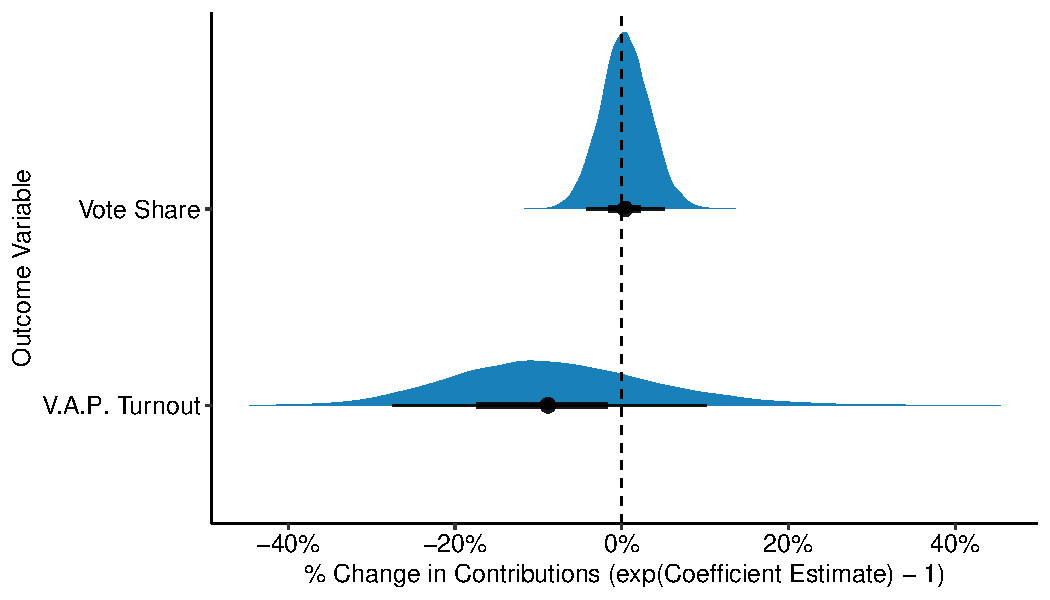
\includegraphics[width=1\linewidth]{../../Figures/Results/vote_coef.pdf}
    \caption{\textbf{The Effect of Rejecting Corporate PAC Contributions on Vote Share and Turnout.} These figures present the posterior distributions estimated for a candidate that pledges to reject corporate PAC contributions. The dot shows the median coefficient estimate, and the intervals show the 50\% and 89\% highest density intervals. This figure shows that rejecting corporate PAC contributions does not affect a candidate's vote percentage or turnout. See Table \ref{tbl: vote results} for the formal estimates.}
    \label{fig: vote coef}
\end{figure*}


\section{Conclusion} \label{sec: conclusion}

The recent trend in Congressional and presidential candidates rejecting corporate PAC contributions is an interesting campaign strategy since campaigns still require a large amount of money to be successful. Although candidates advertise this strategy as an attempt to finance their campaigns with small-dollar individual donations, it is unclear how it affects funding from other sources. 

Using campaign finance data for a sample of 2018 Democratic Congressional candidates who won their election, I find that rejecting corporate PAC contributions decrease the total amount of contributions candidates receive from business PACs, as expected. Rejecting corporate PAC contributions is also associated with an increase in individual contributions less than \$200 as candidates hope for. 

From the perspective of making campaign financing more transparent, the strategy of rejecting corporate PAC contributions also has less desirable effects, however. Candidates who pursue this strategy also receive more contributions from elected officials, individuals affiliated with ideological interest groups, individuals affiliated with businesses, and individual donations greater than \$200. These alternative sources of campaign funds could be indicative of more strategic motivations for rejecting corporate PAC contributions. 

 In some sense, a candidate's decision to reject corporate PAC contributions is obviously strategic since they choose to retain the ability to receive donations from ideological, labor, and political party PACs. Candidates could have also deliberated with these organizations in deciding to announce their opposition to corporate PAC contributions with an agreement that these organizations would help a member's campaign if contributions from individuals fail to reach their expected values. Although directly testing for this strategic behavior is not possible with the data used in this study, the pattern of results are consistent with these possibilities.
 
 Campaign finance reform will likely remain the subject of debate for many years to come. Voters hoping that the growing trend of refusing corporate PAC contributions represents a step toward political transparency and honesty, will, unfortunately, need to reevaluate those hopes. Such a strategy could be a step toward these goals, but it is also associated with individuals making contributions to influence politics in less transparent ways. 


\pagebreak
\singlespacing
\pdfbookmark[1]{References}{References}
%\bibliography{/Users/nick/Documents/Research/Articles/reference.bib}
\printbibliography
\pagebreak


\begin{appendices}
\doublespacing
% Set Tables Names to have "A" Before the Table Names
\setcounter{table}{0}
\renewcommand{\thetable}{A\arabic{table}}

\section{Results Tables}


\begin{table}[h]
\begin{center}
\caption{The Effects of Pledging to Reject Corporate PAC contributions on Contributions from PACs}
\label{tbl: pac results}
\resizebox{\columnwidth}{!}{%
\setlength{\linewidth}{.1cm}\newcommand{\contents}{\begin{tabular}{@{\extracolsep{5pt}}l c c c c }
 \\[-1.8ex] \toprule  \\[-1.8ex]
 & \multicolumn{4}{c}{\textbf{Outcome Variable:}} \\
\textbf{Predictor Variables} & Total PAC \$ & Business PAC \$ & Ideological PAC \$ & Labor PAC \$ \\
 \midrule  \\[-1.8ex]
\\[-1.8ex] \textit{Gamma Model (log link)} \\
\midrule  \\[-1.8ex]
 \\[-1.8ex] \textit{Predictor of Interest} \\  \\[-1.8ex]
	\quad No to Corporate PAC Contributions     & $-0.79^{*}$               & $-2.02^{*}$               & $-0.13^{*}$             & $-0.51^{*}$             \\
          & $[-0.84;\ -0.74]$         & $[-2.17;\ -1.88]$         & $[-0.18;\ -0.06]$       & $[-0.57;\ -0.45]$       \\
\\[-1.8ex] \textit{Controls} \\ \\[-1.8ex]
	\quad New Member    & $-1.04^{*}$               & $-2.41^{*}$               & $0.68^{*}$              & $-0.41^{*}$             \\
          & $[-1.07;\ -1.00]$         & $[-2.49;\ -2.32]$         & $[0.61;\ 0.74]$         & $[-0.46;\ -0.36]$       \\
	\quad \% of White Population in District  & $-0.00$                   & $-0.01^{*}$               & $-0.04^{*}$             & $0.01^{*}$              \\
          & $[-0.00;\ 0.00]$          & $[-0.01;\ -0.01]$         & $[-0.05;\ -0.03]$       & $[0.01;\ 0.02]$         \\
	\quad \% of Black Population in District  & $-0.00$                   & $-0.00^{*}$               & $-0.04^{*}$             & $0.00$                  \\
          & $[-0.01;\ 0.00]$          & $[-0.01;\ -0.00]$         & $[-0.05;\ -0.04]$       & $[-0.01;\ 0.01]$        \\
	\quad \% of Latino Population in District & $-0.00$                   & $-0.01^{*}$               & $-0.03^{*}$             & $0.00$                  \\
          & $[-0.01;\ 0.00]$          & $[-0.01;\ -0.01]$         & $[-0.03;\ -0.02]$       & $[-0.00;\ 0.01]$        \\
	\quad \% of Asian Population in District  & $-0.02^{*}$               & $-0.01^{*}$               & $-0.05^{*}$             & $-0.01^{*}$             \\
          & $[-0.02;\ -0.02]$         & $[-0.02;\ -0.01]$         & $[-0.06;\ -0.04]$       & $[-0.01;\ -0.00]$       \\
	\quad \% of District Pop. with Bachelors Degree   & $-0.01^{*}$               & $-0.01^{*}$               & $0.00$                  & $-0.01^{*}$             \\
          & $[-0.01;\ -0.01]$         & $[-0.01;\ -0.01]$         & $[-0.00;\ 0.01]$        & $[-0.02;\ -0.01]$       \\
	\quad \% of District Vote for Clinton in 2016  & $-0.02^{*}$               & $-0.03^{*}$               & $-0.02^{*}$             & $0.01^{*}$              \\
          & $[-0.02;\ -0.01]$         & $[-0.03;\ -0.03]$         & $[-0.03;\ -0.02]$       & $[0.01;\ 0.02]$         \\
	\quad \% of District Vote for Dem. House Candidates in 2016  & $0.01^{*}$                & $0.01^{*}$                & $-0.00$                 & $-0.00^{*}$             \\
          & $[0.00;\ 0.01]$           & $[0.01;\ 0.01]$           & $[-0.00;\ 0.00]$        & $[-0.00;\ -0.00]$       \\
	\quad $\log$(Voting Age Population in District)   & $0.15$                    & $-0.05$                   & $1.32^{*}$              & $0.07$                  \\
          & $[-0.03;\ 0.33]$          & $[-0.28;\ 0.18]$          & $[0.83;\ 1.79]$         & $[-0.18;\ 0.30]$        \\
		\quad $\log$(Median Household Income)    & $0.64^{*}$                & $0.59^{*}$                & $0.29^{*}$              & $0.02$                  \\
          & $[0.57;\ 0.72]$           & $[0.50;\ 0.69]$           & $[0.10;\ 0.49]$         & $[-0.08;\ 0.13]$        \\
	\quad Intercept         & $13.33^{*}$               & $12.93^{*}$               & $10.07^{*}$             & $11.67^{*}$             \\
          & $[13.32;\ 13.34]$         & $[12.92;\ 12.95]$         & $[10.04;\ 10.10]$       & $[11.66;\ 11.69]$       \\ 
Dispersion Parameter     & $2514.54^{*}$             & $2363.02^{*}$             & $974.90^{*}$            & $1018.48^{*}$           \\
          & $[2475.14;\ 2554.93]$     & $[2323.03;\ 2400.76]$     & $[951.17;\ 1000.97]$    & $[992.44;\ 1043.38]$    \\
\\[-1.8ex] \textit{Binomial Model (Logit Link)} \\
\midrule  \\[-1.8ex]
\\[-1.8ex] \textit{Predictor of Interest} \\ \\[-1.8ex]
	\quad No to Corporate PAC Contributions     & $0.24$                    & $1.41^{*}$                & $-0.13$                 & $-0.00$                 \\
          & $[-1.07;\ 1.54]$          & $[0.43;\ 2.29]$           & $[-1.35;\ 1.14]$        & $[-0.20;\ 0.20]$        \\
\\[-1.8ex] \textit{Controls} \\ \\[-1.8ex]
	\quad New Member    & $-0.81$                   & $0.76$                    & $0.24$                  & $-0.01$                 \\
          & $[-2.19;\ 0.43]$          & $[-0.17;\ 1.69]$          & $[-0.89;\ 1.40]$        & $[-0.18;\ 0.16]$        \\
	\quad Intercept         & $-3.56^{*}$               & $-3.34^{*}$               & $-3.54^{*}$             & $-3.70^{*}$             \\
          & $[-4.33;\ -2.87]$         & $[-4.00;\ -2.70]$         & $[-4.28;\ -2.85]$       & $[-3.77;\ -3.63]$       \\
          \\
 \midrule  \\[-1.8ex]
Number of Observations & 167 & 167 & 167 & 167 \\
\bottomrule  \\[-1.8ex]
\multicolumn{5}{p{\linewidth}}{Notes: Models are estimated using zero-augmented Gamma likelihoods. Analyses use four Markov chain Monte Carlo (MCMC) chains at 10,000 iterations each with a warmup period of 5,000 samples using the Hamiltonian Monte Carlo algorithm. All chains indicate convergence with every \^{R} value being less than 1.01. Model coefficients are estimated with weakly informative priors. 89\% highest density intervals shown in brackets below each coefficient. $^*$ indicates that 0 is outside 89\% highest posterior density interval.}\\
\end{tabular}}
\setbox0=\hbox{\contents}
	\setlength{\linewidth}{\wd0-2\tabcolsep-.25em}
	\contents
}
\end{center}
\end{table}



\begin{table}[h]
\begin{center}
\caption{The Effects of Pledging to Reject Corporate PAC contributions on Contributions from Party Organizations}
\label{tbl: party results}
\resizebox{\columnwidth}{!}{%
\setlength{\linewidth}{.1cm}\newcommand{\contents}{\begin{tabular}{@{\extracolsep{5pt}}l c c c }
 \\[-1.8ex] \toprule  \\[-1.8ex]
 & \multicolumn{3}{c}{\textbf{Outcome Variable:}} \\
\textbf{Predictor Variables} & Leadership PAC \$ & Candidate Committee PAC \$ & Party Committee \$ \\
 \midrule  \\[-1.8ex]
\\[-1.8ex] \textit{Gamma Model (log link)} \\
\midrule  \\[-1.8ex]
 \\[-1.8ex] \textit{Predictor of Interest} \\  \\[-1.8ex]
\quad No to Corporate PAC Contributions     & $-0.23^{*}$             & $0.12^{*}$              & $-0.08$               \\
          & $[-0.31;\ -0.15]$       & $[0.02;\ 0.22]$         & $[-0.22;\ 0.04]$      \\
\\[-1.8ex] \textit{Controls} \\ \\[-1.8ex]
	\quad New Member    & $1.24^{*}$              & $0.63^{*}$              & $0.04$                \\
          & $[1.14;\ 1.34]$         & $[0.51;\ 0.75]$         & $[-0.11;\ 0.18]$      \\
\quad \% of White Population in District   & $-0.07^{*}$             & $-0.02$                 & $0.51^{*}$            \\
          & $[-0.08;\ -0.06]$       & $[-0.04;\ 0.00]$        & $[0.43;\ 0.58]$       \\
\quad \% of Black Population in District  & $-0.08^{*}$             & $-0.01$                 & $0.53^{*}$            \\
          & $[-0.09;\ -0.07]$       & $[-0.03;\ 0.00]$        & $[0.45;\ 0.61]$       \\
\quad \% of Latino Population in District & $-0.07^{*}$             & $-0.01$                 & $0.54^{*}$            \\
          & $[-0.08;\ -0.06]$       & $[-0.03;\ 0.01]$        & $[0.47;\ 0.62]$       \\
\quad \% of Asian Population in District  & $-0.11^{*}$             & $-0.02$                 & $0.49^{*}$            \\
          & $[-0.13;\ -0.10]$       & $[-0.04;\ 0.00]$        & $[0.39;\ 0.60]$       \\
\quad \% of District Pop. with Bachelors Degree   & $-0.02^{*}$             & $-0.02^{*}$             & $0.01$                \\
          & $[-0.03;\ -0.02]$       & $[-0.03;\ -0.02]$       & $[-0.01;\ 0.02]$      \\
\quad \% of District Vote for Clinton in 2016  & $-0.01^{*}$             & $-0.02^{*}$             & $-0.13^{*}$           \\
          & $[-0.02;\ -0.00]$       & $[-0.02;\ -0.01]$       & $[-0.15;\ -0.10]$     \\
\quad \% of District Vote for Dem. House Candidates in 2016  & $-0.01^{*}$             & $-0.01^{*}$             & $-0.00$               \\
          & $[-0.02;\ -0.01]$       & $[-0.01;\ -0.01]$       & $[-0.01;\ 0.00]$      \\
\quad $\log$(Voting Age Population in District)   & $3.34^{*}$              & $2.39^{*}$              & $-0.41$               \\
          & $[2.71;\ 3.93]$         & $[1.70;\ 3.07]$         & $[-2.04;\ 1.22]$      \\
\quad $\log$(Median Household Income)    & $1.42^{*}$              & $0.74^{*}$              & $-0.07$               \\
          & $[1.13;\ 1.71]$         & $[0.41;\ 1.05]$         & $[-0.79;\ 0.66]$      \\
\quad Intercept         & $9.30^{*}$              & $8.58^{*}$              & $6.61^{*}$            \\
          & $[9.24;\ 9.35]$         & $[8.53;\ 8.64]$         & $[6.45;\ 6.79]$       \\
Dispersion Parameter     & $1113.08^{*}$           & $572.91^{*}$            & $68.92^{*}$           \\
          & $[1087.71;\ 1141.14]$   & $[553.86;\ 591.51]$     & $[62.54;\ 75.63]$     \\
\\[-1.8ex] \textit{Binomial Model (Logit Link)} \\
\midrule  \\[-1.8ex]
\\[-1.8ex] \textit{Predictor of Interest} \\ \\[-1.8ex]
\quad No to Corporate PAC Contributions     & $0.13$                  & $0.41$                  & $-0.01$               \\
          & $[-0.89;\ 1.08]$        & $[-0.48;\ 1.32]$        & $[-0.80;\ 0.83]$      \\
\\[-1.8ex] \textit{Controls} \\ \\[-1.8ex]
	\quad New Member     & $-0.55$                 & $-0.35$                 & $-1.13^{*}$           \\
          & $[-1.54;\ 0.36]$        & $[-1.24;\ 0.48]$        & $[-1.87;\ -0.41]$     \\
\quad Intercept         & $-2.05^{*}$             & $-1.92^{*}$             & $2.00^{*}$            \\
          & $[-2.47;\ -1.61]$       & $[-2.33;\ -1.51]$       & $[1.58;\ 2.42]$       \\
          \\
 \midrule  \\[-1.8ex]
Number of Observations & 167 & 167 & 167 \\
\bottomrule  \\[-1.8ex]
\multicolumn{4}{p{\linewidth}}{Notes: Models are estimated using zero-augmented Gamma likelihoods. Analyses use four Markov chain Monte Carlo (MCMC) chains at 10,000 iterations each with a warmup period of 5,000 samples using the Hamiltonian Monte Carlo algorithm. All chains indicate convergence with every \^{R} value being less than 1.01. Model coefficients are estimated with weakly informative priors. 89\% highest density intervals shown in brackets below each coefficient. $^*$ indicates that 0 is outside 89\% highest posterior density interval.}
\end{tabular}}
\setbox0=\hbox{\contents}
	\setlength{\linewidth}{\wd0-2\tabcolsep-.25em}
	\contents
}
\end{center}
\end{table}


\begin{landscape}

\begin{table}
\begin{center}
\begin{tabular}{l c c c c c }
\hline
 & Model 1 & Model 2 & Model 3 & Model 4 & Model 5 \\
\hline
a         & $10.87^{*}$           & $13.12^{*}$           & $13.26^{*}$           & $10.27^{*}$           & $12.48^{*}$           \\
          & $[10.84;\ 10.91]$     & $[13.11;\ 13.13]$     & $[13.25;\ 13.28]$     & $[10.23;\ 10.31]$     & $[12.46;\ 12.49]$     \\
b\_np     & $0.65^{*}$            & $0.26^{*}$            & $0.34^{*}$            & $0.27^{*}$            & $0.08^{*}$            \\
          & $[0.61;\ 0.69]$       & $[0.24;\ 0.28]$       & $[0.32;\ 0.36]$       & $[0.21;\ 0.32]$       & $[0.05;\ 0.12]$       \\
b\_new    & $0.99^{*}$            & $0.63^{*}$            & $0.69^{*}$            & $0.63^{*}$            & $0.14^{*}$            \\
          & $[0.94;\ 1.04]$       & $[0.60;\ 0.66]$       & $[0.66;\ 0.71]$       & $[0.56;\ 0.70]$       & $[0.10;\ 0.18]$       \\
b\_white  & $-0.04^{*}$           & $-0.01^{*}$           & $-0.01^{*}$           & $-0.06^{*}$           & $-0.00$               \\
          & $[-0.04;\ -0.03]$     & $[-0.01;\ -0.00]$     & $[-0.01;\ -0.01]$     & $[-0.07;\ -0.05]$     & $[-0.01;\ 0.00]$      \\
b\_black  & $-0.08^{*}$           & $-0.02^{*}$           & $-0.03^{*}$           & $-0.08^{*}$           & $-0.01^{*}$           \\
          & $[-0.09;\ -0.08]$     & $[-0.02;\ -0.02]$     & $[-0.03;\ -0.02]$     & $[-0.09;\ -0.07]$     & $[-0.02;\ -0.01]$     \\
b\_latino & $-0.04^{*}$           & $0.00$                & $-0.00$               & $-0.04^{*}$           & $0.01^{*}$            \\
          & $[-0.04;\ -0.03]$     & $[-0.00;\ 0.01]$      & $[-0.00;\ 0.00]$      & $[-0.05;\ -0.04]$     & $[0.00;\ 0.01]$       \\
b\_asian  & $-0.06^{*}$           & $-0.02^{*}$           & $-0.02^{*}$           & $-0.10^{*}$           & $-0.02^{*}$           \\
          & $[-0.06;\ -0.05]$     & $[-0.03;\ -0.02]$     & $[-0.03;\ -0.02]$     & $[-0.11;\ -0.09]$     & $[-0.02;\ -0.01]$     \\
b\_bach   & $-0.01^{*}$           & $-0.02^{*}$           & $-0.01^{*}$           & $-0.03^{*}$           & $-0.02^{*}$           \\
          & $[-0.01;\ -0.01]$     & $[-0.02;\ -0.01]$     & $[-0.02;\ -0.01]$     & $[-0.03;\ -0.02]$     & $[-0.02;\ -0.01]$     \\
b\_mhh    & $1.70^{*}$            & $2.14^{*}$            & $2.02^{*}$            & $3.66^{*}$            & $2.35^{*}$            \\
          & $[1.57;\ 1.84]$       & $[2.07;\ 2.20]$       & $[1.95;\ 2.09]$       & $[3.47;\ 3.86]$       & $[2.25;\ 2.44]$       \\
b\_clint  & $0.00^{*}$            & $-0.01^{*}$           & $-0.00^{*}$           & $0.01^{*}$            & $-0.01^{*}$           \\
          & $[0.00;\ 0.01]$       & $[-0.01;\ -0.00]$     & $[-0.00;\ -0.00]$     & $[0.01;\ 0.02]$       & $[-0.01;\ -0.01]$     \\
b\_house  & $-0.02^{*}$           & $-0.01^{*}$           & $-0.01^{*}$           & $-0.02^{*}$           & $-0.01^{*}$           \\
          & $[-0.02;\ -0.01]$     & $[-0.01;\ -0.01]$     & $[-0.01;\ -0.01]$     & $[-0.02;\ -0.02]$     & $[-0.01;\ -0.01]$     \\
b\_vpop   & $-1.01^{*}$           & $0.29^{*}$            & $0.15$                & $2.03^{*}$            & $1.15^{*}$            \\
          & $[-1.39;\ -0.61]$     & $[0.10;\ 0.46]$       & $[-0.03;\ 0.31]$      & $[1.58;\ 2.44]$       & $[0.93;\ 1.37]$       \\
scale     & $2269.85^{*}$         & $3736.92^{*}$         & $4093.72^{*}$         & $1590.11^{*}$         & $2658.66^{*}$         \\
          & $[2231.85;\ 2307.67]$ & $[3688.43;\ 3786.97]$ & $[4042.18;\ 4142.89]$ & $[1559.51;\ 1622.18]$ & $[2617.17;\ 2699.15]$ \\
prob      & $0.01^{*}$            & $0.01^{*}$            & $0.01^{*}$            & $0.05^{*}$            & $0.01^{*}$            \\
          & $[0.00;\ 0.02]$       & $[0.00;\ 0.02]$       & $[0.00;\ 0.02]$       & $[0.02;\ 0.08]$       & $[0.00;\ 0.02]$       \\
\hline
\multicolumn{6}{l}{\scriptsize{$^*$ 0 outside 89\% highest posterior density interval}}
\end{tabular}
\caption{Statistical models}
\label{table:coefficients}
\end{center}
\end{table}

\end{landscape}


\begin{table}[!htb]
\begin{center}
\caption{The Effects of Pledging to Reject Corporate PAC contributions on Voter Support}
\label{tbl: vote results}
\resizebox{\columnwidth}{!}{%
\setlength{\linewidth}{.1cm}\newcommand{\contents}{\begin{tabular}{@{\extracolsep{5pt}}l c c }
 \\[-1.8ex] \toprule  \\[-1.8ex]
 & \multicolumn{2}{c}{\textbf{Outcome Variable:}} \\
\textbf{Predictor Variables} & Candidate Vote \% & Voting Age Population Turnout \% \\
 \midrule  \\[-1.8ex]
\\[-1.8ex] \textit{Gamma Model (log link)} \\
\midrule  \\[-1.8ex]
 \\[-1.8ex] \textit{Predictor of Interest} \\  \\[-1.8ex]
\quad No to Corporate PAC Contributions     & $0.00$            & $-0.09$           \\
          & $[-0.04;\ 0.05]$  & $[-0.30;\ 0.12]$  \\
\\[-1.8ex] \textit{Controls} \\ \\[-1.8ex]
	\quad New Member    & $-0.09^{*}$       & $0.14$            \\
          & $[-0.13;\ -0.04]$ & $[-0.08;\ 0.35]$  \\
\quad \% of White Population in District  & $0.00$            & $-0.01$           \\
          & $[-0.00;\ 0.01]$  & $[-0.03;\ 0.02]$  \\
\quad \% of Black Population in District  & $0.00$            & $-0.03^{*}$       \\
          & $[-0.00;\ 0.01]$  & $[-0.05;\ -0.00]$ \\
\quad \% of Latino Population in District & $0.00$            & $-0.03^{*}$       \\
          & $[-0.00;\ 0.01]$  & $[-0.06;\ -0.01]$ \\
\quad \% of Asian Population in District   & $0.00$            & $-0.02$           \\
          & $[-0.00;\ 0.01]$  & $[-0.05;\ 0.01]$  \\
\quad \% of District Pop. with Bachelors Degree   & $0.00$            & $-0.02^{*}$       \\
          & $[-0.00;\ 0.00]$  & $[-0.03;\ -0.00]$ \\
\quad \% of District Vote for Clinton in 2016  & $0.01^{*}$        & $0.04^{*}$        \\
          & $[0.01;\ 0.01]$   & $[0.02;\ 0.05]$   \\
\quad \% of District Vote for Dem. House Candidates in 2016  & $0.00$            & $-0.01^{*}$       \\
          & $[-0.00;\ 0.00]$  & $[-0.02;\ -0.00]$ \\
\quad $\log$(Voting Age Population in District)   & $0.02$            & $-1.74^{*}$       \\
          & $[-0.27;\ 0.32]$  & $[-3.14;\ -0.34]$ \\
\quad $\log$(Median Household Income)    & $-0.10$           & $0.73^{*}$        \\
          & $[-0.21;\ 0.00]$  & $[0.17;\ 1.28]$   \\
\quad Intercept         & $4.22^{*}$        & $3.28^{*}$        \\
          & $[4.20;\ 4.24]$   & $[3.19;\ 3.36]$   \\
Dispersion Parameter     & $0.79^{*}$        & $8.67^{*}$        \\
          & $[0.65;\ 0.94]$   & $[7.14;\ 10.40]$  \\
\midrule  \\[-1.8ex]
Number of Observations & 167 & 167 \\
\bottomrule  \\[-1.8ex]
\multicolumn{3}{p{\linewidth}}{Notes: Models are estimated using a Gamma likelihood with a log link function. Analyses use four Markov chain Monte Carlo (MCMC) chains at 8,000 iterations each with a warmup period of 3,000 samples using the Hamiltonian Monte Carlo algorithm. All chains indicate convergence with every \^{R} value being less than 1.01. Model coefficients are estimated with weakly informative priors. 89\% highest density intervals shown in brackets below each coefficient. $^*$ indicates that 0 is outside 89\% highest posterior density interval.}
\end{tabular}}
\setbox0=\hbox{\contents}
	\setlength{\linewidth}{\wd0-2\tabcolsep-.25em}
	\contents
}
\end{center}
\end{table}



\section{Prior Simulations} \label{sec: prior sims}

\begin{figure*}[!htb]
    \centering
    \begin{subfigure}[b]{0.45\textwidth}
        \centering
        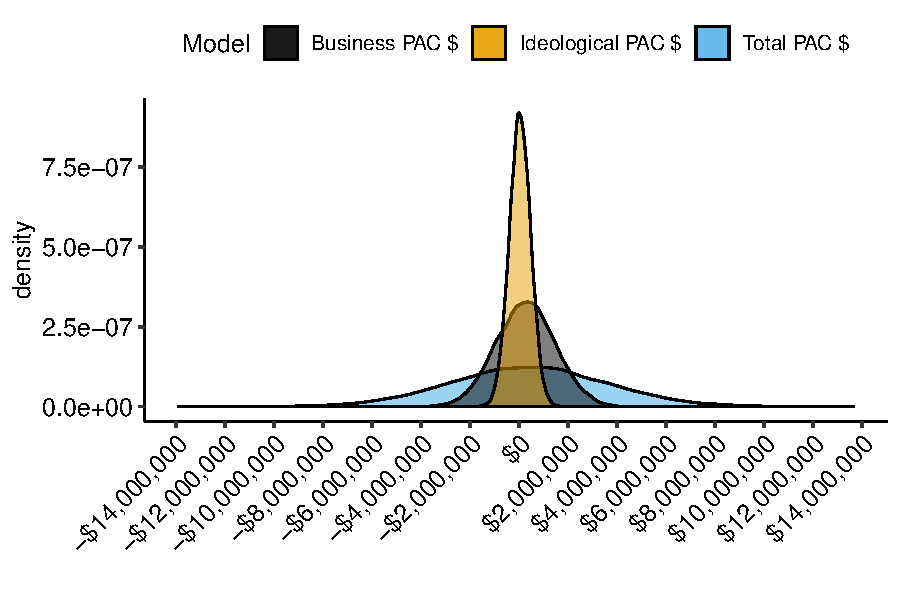
\includegraphics[width=\linewidth]{../../Figures/Priors/pac_int.pdf}
        \caption{Priors for Model Intercepts}
    \end{subfigure}
    %
    \begin{subfigure}[b]{0.45\textwidth}
        \centering
        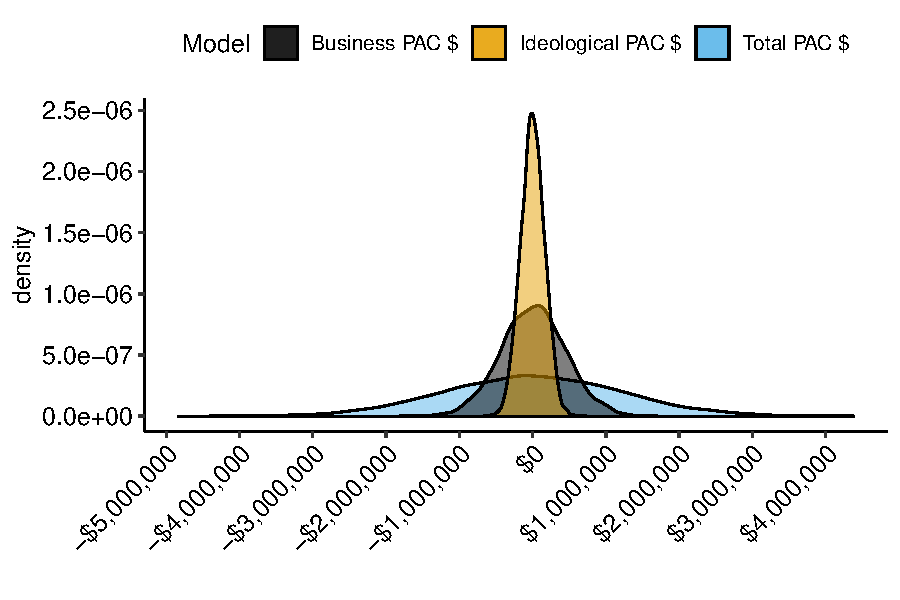
\includegraphics[width=\linewidth]{../../Figures/Priors/pac_slopes.pdf}
        \caption{Priors for Model Slopes}
    \end{subfigure}
    %
    \begin{subfigure}[b]{0.45\textwidth}
    	\centering
        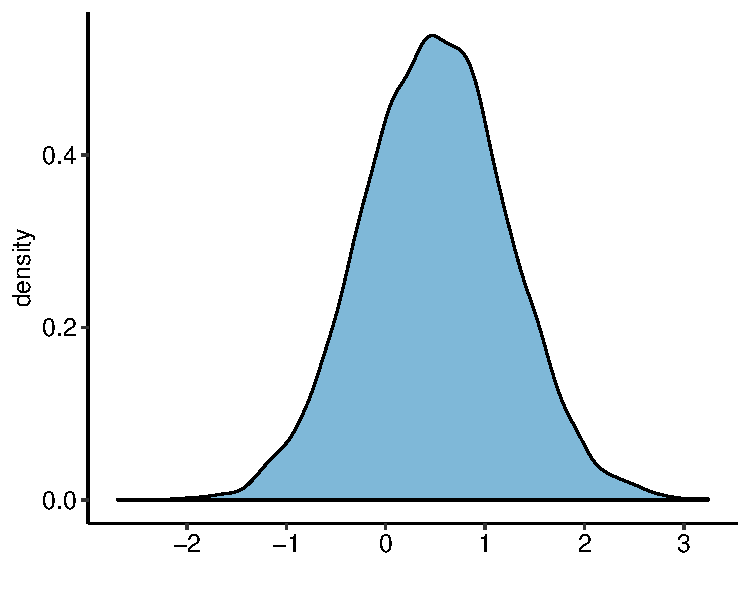
\includegraphics[width=\linewidth]{../../Figures/Priors/pac_logit.pdf}
        \caption{Binomial Intercept \& Slope Priors}
    \end{subfigure}
    %
    \begin{subfigure}[b]{0.45\textwidth}
    	\centering
        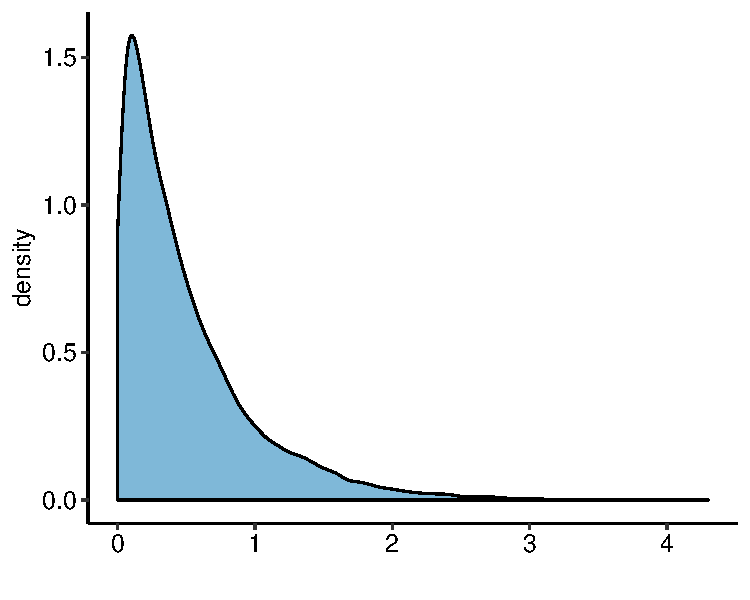
\includegraphics[width=\linewidth]{../../Figures/Priors/pac_scale.pdf}
        \caption{Scale Parameter Priors}
    \end{subfigure}
    \caption{\textbf{Priors for Parameters in PAC Contribution Models.}}
    \label{fig: priors}
\end{figure*}

\begin{figure*}[!htb]
    \centering
    \begin{subfigure}[b]{0.45\textwidth}
        \centering
        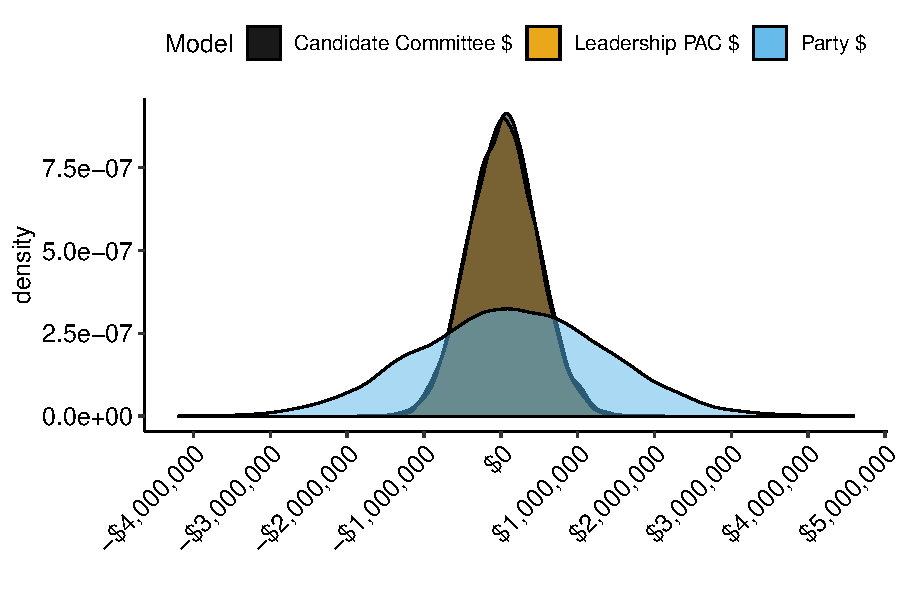
\includegraphics[width=\linewidth]{../../Figures/Priors/party_int.pdf}
        \caption{Priors for Model Intercepts}
    \end{subfigure}
    %
    \begin{subfigure}[b]{0.45\textwidth}
        \centering
        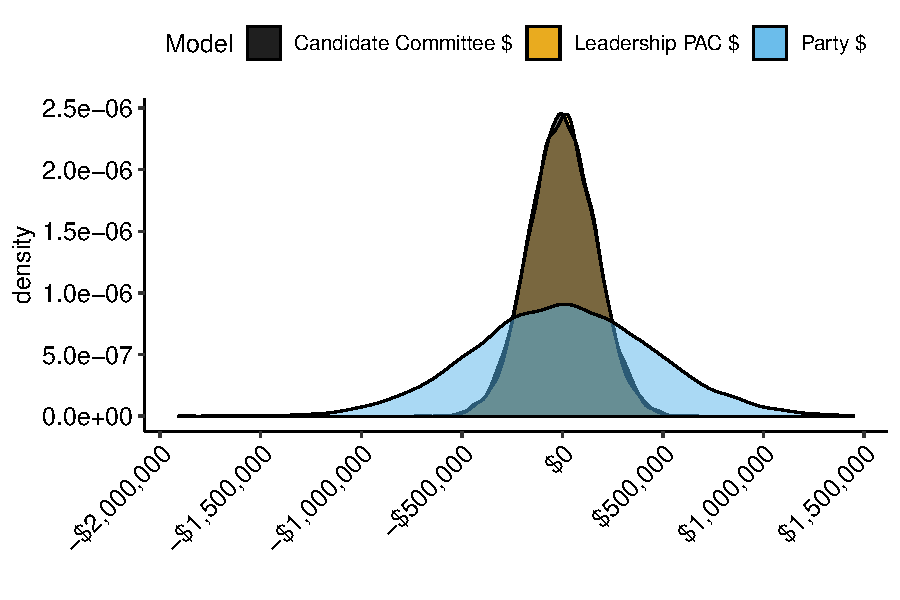
\includegraphics[width=\linewidth]{../../Figures/Priors/party_slopes.pdf}
        \caption{Priors for Model Slopes}
    \end{subfigure}
    %
    \begin{subfigure}[b]{0.45\textwidth}
    	\centering
        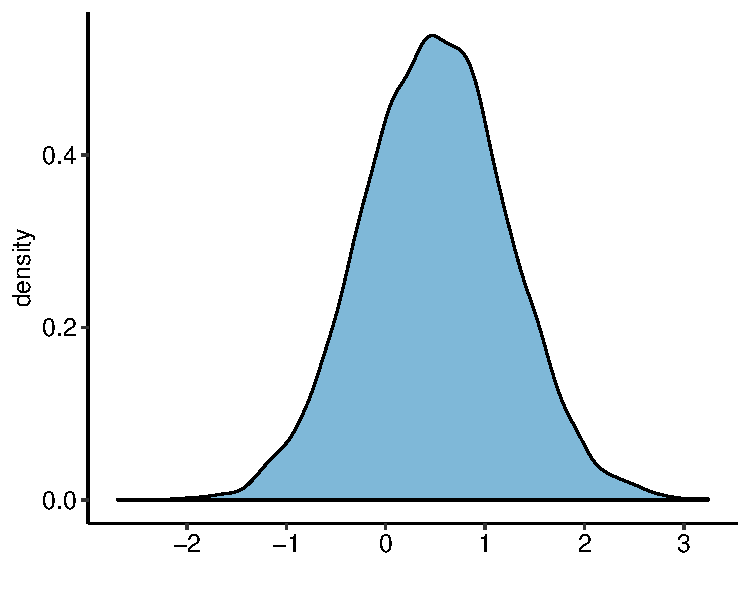
\includegraphics[width=\linewidth]{../../Figures/Priors/pac_logit.pdf}
        \caption{Binomial Intercept \& Slope Priors}
    \end{subfigure}
    %
    \begin{subfigure}[b]{0.45\textwidth}
    	\centering
        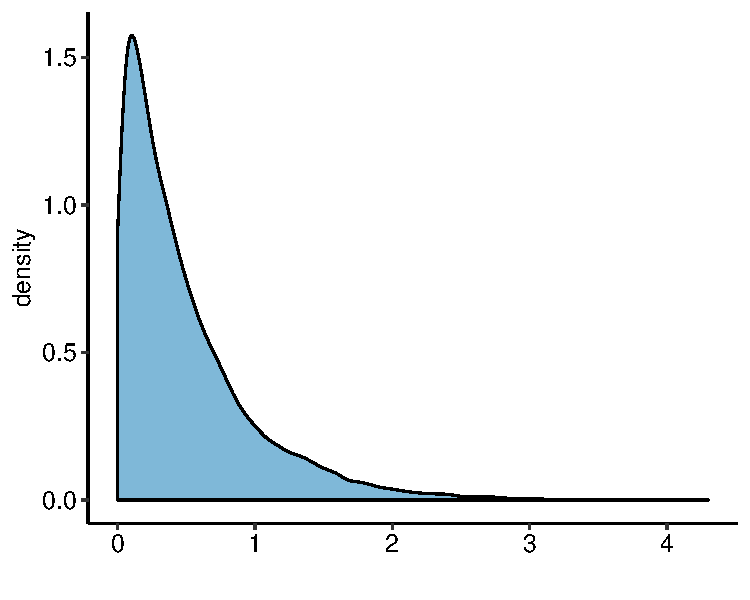
\includegraphics[width=\linewidth]{../../Figures/Priors/pac_scale.pdf}
        \caption{Scale Parameter Priors}
    \end{subfigure}
    \caption{\textbf{Priors for Parameters in Political Party Contribution Models.}}
    \label{fig: priors}
\end{figure*}

\begin{figure*}[!htb]
    \centering
    \begin{subfigure}[b]{0.45\textwidth}
        \centering
        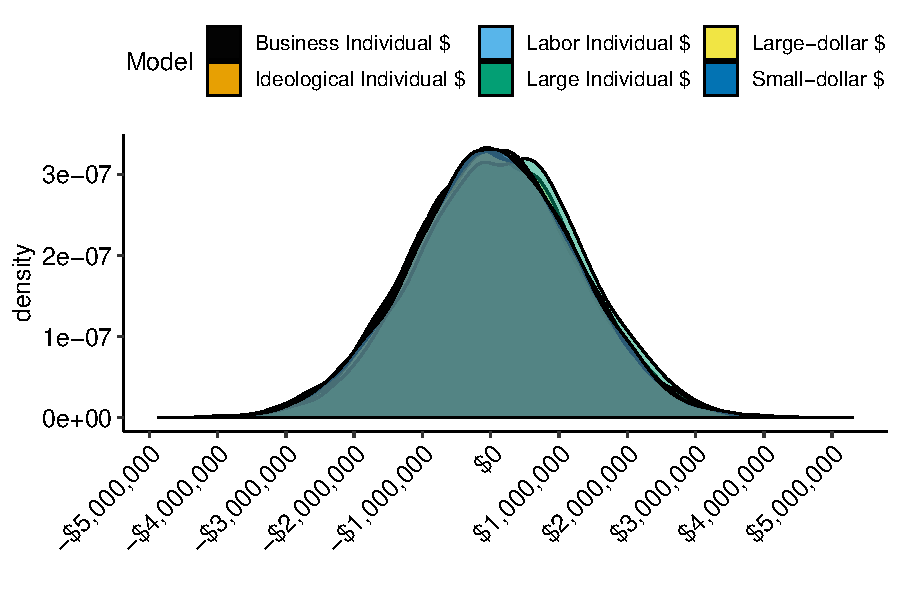
\includegraphics[width=\linewidth]{../../Figures/Priors/indiv_int.pdf}
        \caption{Priors for Model Intercepts}
    \end{subfigure}
    %
    \begin{subfigure}[b]{0.45\textwidth}
        \centering
        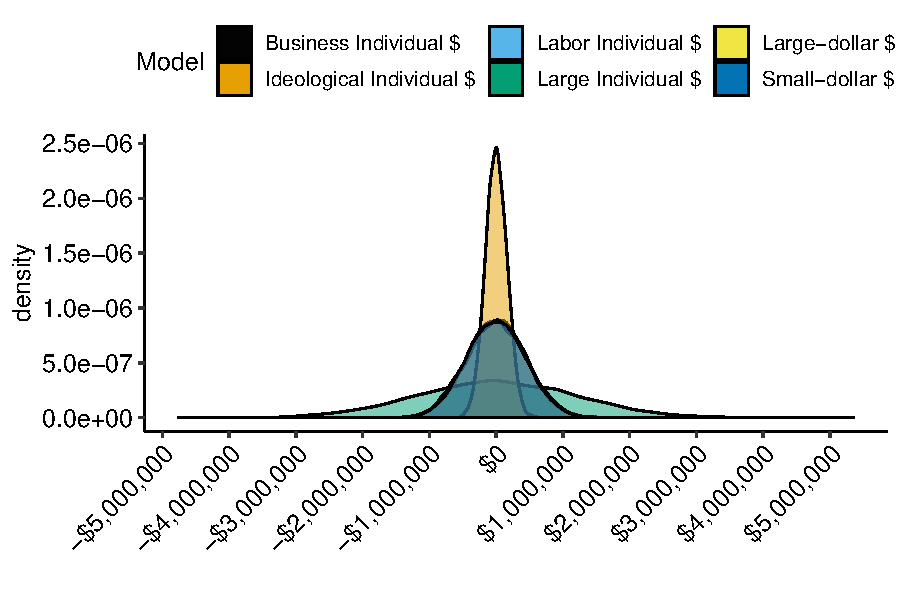
\includegraphics[width=\linewidth]{../../Figures/Priors/indiv_slopes.pdf}
        \caption{Priors for Model Slopes}
    \end{subfigure}
    %
    \begin{subfigure}[b]{0.45\textwidth}
    	\centering
        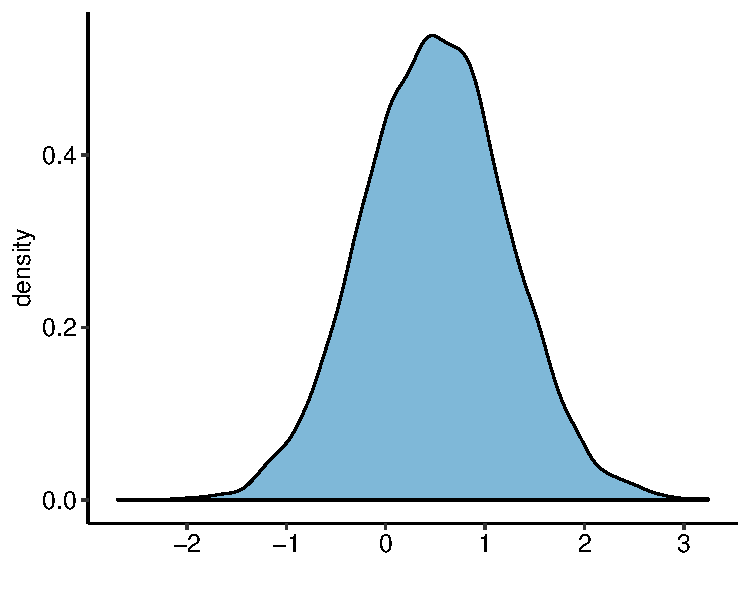
\includegraphics[width=\linewidth]{../../Figures/Priors/pac_logit.pdf}
        \caption{Binomial Intercept \& Slope Priors}
    \end{subfigure}
    %
    \begin{subfigure}[b]{0.45\textwidth}
    	\centering
        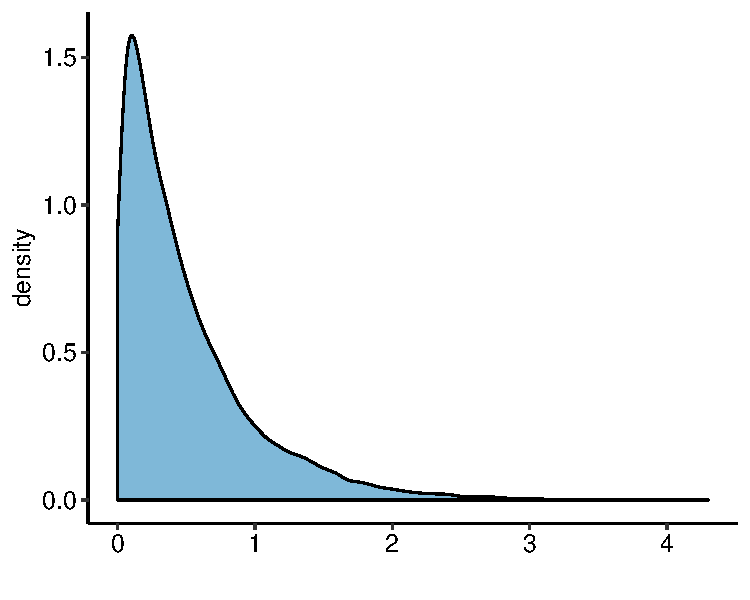
\includegraphics[width=\linewidth]{../../Figures/Priors/pac_scale.pdf}
        \caption{Scale Parameter Priors}
    \end{subfigure}
    \caption{\textbf{Priors for Parameters in Individual Contribution Models.}}
    \label{fig: priors}
\end{figure*}

\begin{figure*}[!htb]
    \centering
    \begin{subfigure}[b]{0.45\textwidth}
        \centering
        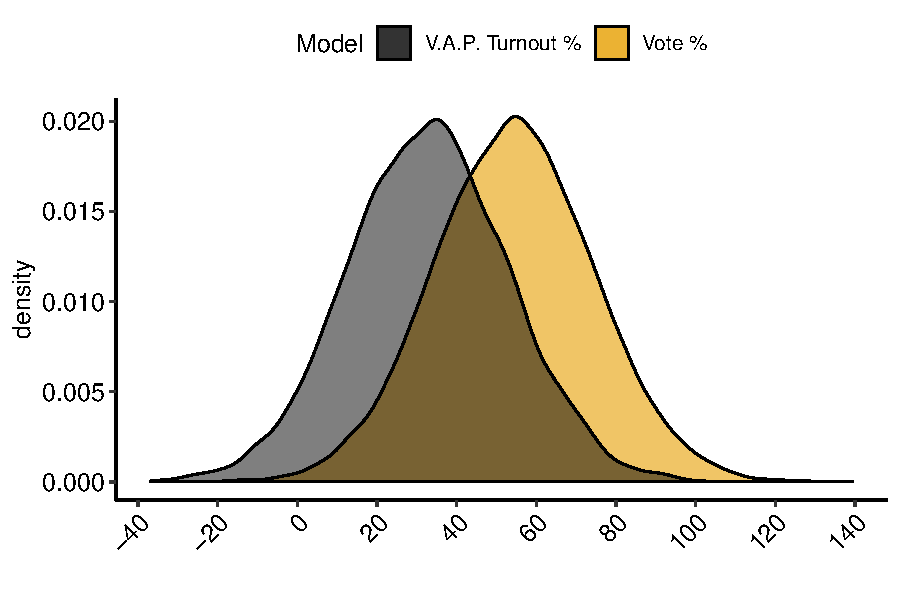
\includegraphics[width=\linewidth]{../../Figures/Priors/vote_int.pdf}
        \caption{Priors for Model Intercepts}
    \end{subfigure}
    %
    \begin{subfigure}[b]{0.45\textwidth}
        \centering
        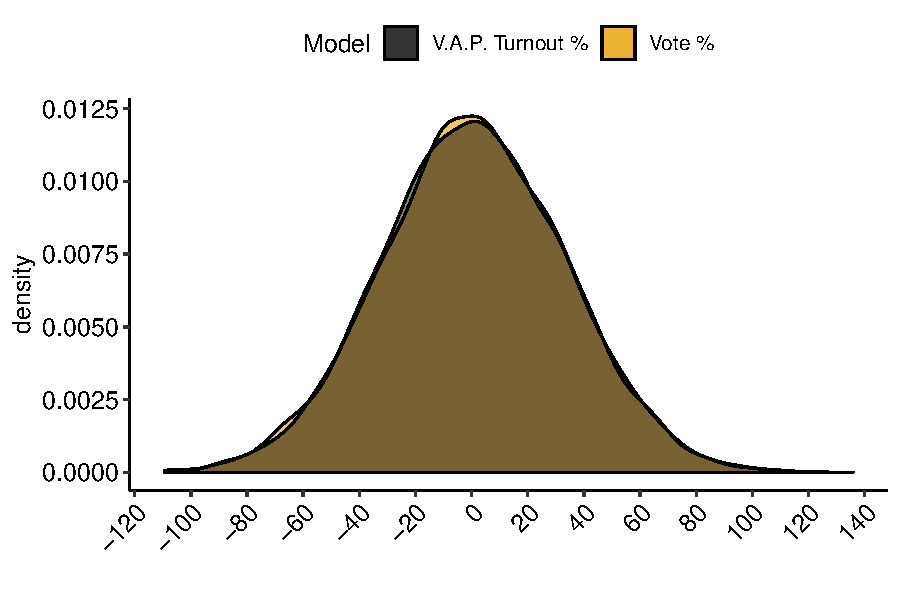
\includegraphics[width=\linewidth]{../../Figures/Priors/vote_slopes.pdf}
        \caption{Priors for Model Slopes}
    \end{subfigure}
    %
    \begin{subfigure}[b]{0.45\textwidth}
    	\centering
        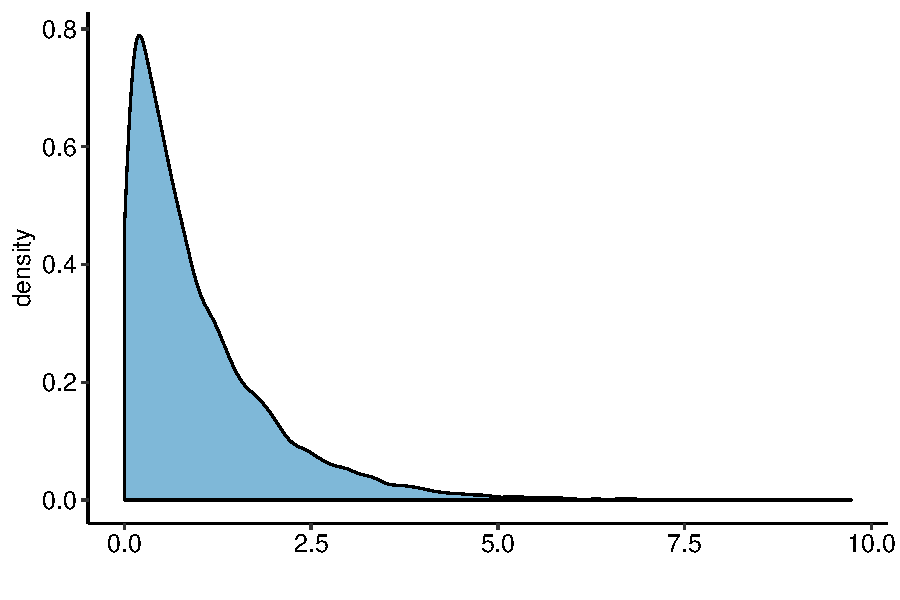
\includegraphics[width=\linewidth]{../../Figures/Priors/vote_scale.pdf}
        \caption{Scale Parameter Priors}
    \end{subfigure}
    \caption{\textbf{Priors for Parameters in Vote Models.}}
    \label{fig: priors}
\end{figure*}


\end{appendices}


\end{document}
